\documentclass[aspectratio=43]{beamer}
% aspectratio=1610,169

\usepackage[czech]{babel}
\usepackage[utf8]{inputenc}
\usepackage[T1]{fontenc}
\usetheme[workplace=sci,]{MU}
\usepackage{tikz}
\usepackage{scalerel}
\usepackage{tcolorbox}
\usepackage{xcolor}
\usepackage{bbding}
\usepackage{pifont}
\usepackage{wasysym}
\usepackage{amssymb}
\usepackage{rotating}
\usepackage{shadowtext}

\usetikzlibrary{arrows.meta, positioning}
\usetikzlibrary{matrix,calc}

\definecolor{myblack}{RGB}{24,24,24}
\definecolor{myblue}{RGB}{61,13,255}
\definecolor{myred}{RGB}{255,2,2}
\definecolor{mygreen}{RGB}{51,255,0}
\definecolor{myyellow}{RGB}{235,255,0}
\definecolor{pressure}{RGB}{31,119,180}
\definecolor{volume}{RGB}{255,127,14}
% \definecolor{darktangerine}{rgb}{1.0, 0.66, 0.07}
\definecolor{mybluee}{RGB}{33,141,232}
\definecolor{darktangerine}{RGB}{229,173,78}
\definecolor{myredd}{RGB}{204,14,14}

\def\vs{\vspace{-2mm}}
\def\lend{\phantom{g}\vspace{1.5mm}\hrule\hrule}

\setbeamercolor{normal text}{fg=black,bg=white}
\setbeamertemplate{sidebar right}{}
\useoutertheme[subsection=false]{miniframes}
\setbeamertemplate{footline}{\begin{flushright} \bf \insertframenumber{}$\,$/$\,$\inserttotalframenumber \hphantom{aaa.}\end{flushright}\vspace{-0.11cm}}

% \addtobeamertemplate{alerted text begin}{\setbeamercolor{item}{fg=alerted text.fg}}{}
\setbeamercolor{alerted text}{fg=black}

\date{}

\begin{document}


\begin{frame}[noframenumbering,plain]
\begin{tikzpicture}[remember picture,overlay,shift={(current page.center)}]
    \draw (0, 0) node[fill opacity=0.53] {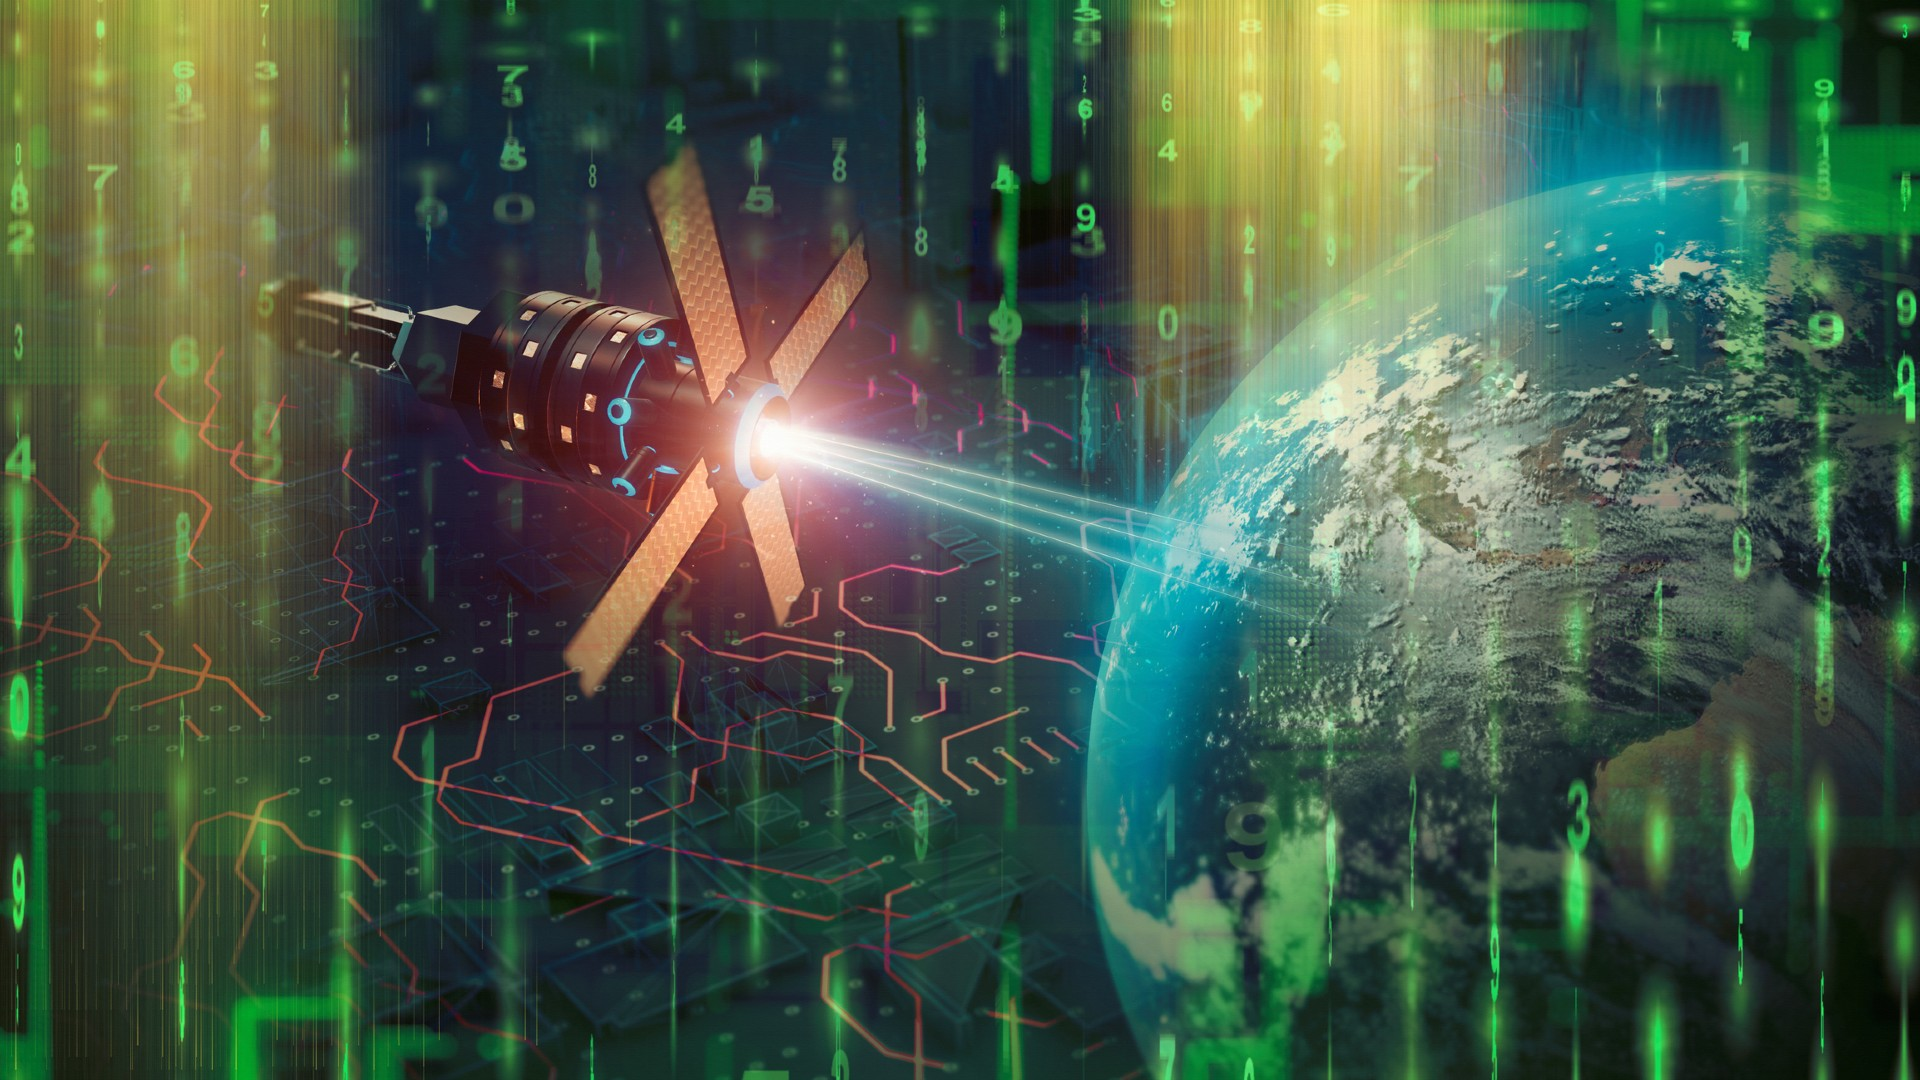
\includegraphics[width=1.5\linewidth]{AI/ai_in_astronomy2.jpg}};
    
    \draw (-3.95, 3.85) node {
\includegraphics[height=35pt]{mubeamer/logo/mubeamer-sci-english-color.pdf}};
    \draw (4.05, 3.85) node {
\includegraphics[height=26pt]{mubeamer/label/mubeamer-mu-czech.pdf}};

    \draw (0, 1.05) node {\Huge \color{black} \bf Využití umělé inteligence};
    \draw (0, 0.05) node {\Huge \color{black} \bf v astronomii};
    \draw (0, -1.95) node {\Large \color{black} \textbf{Tomáš Plšek}};

    \draw (-5.95, -4.43) node[right] {\small \color{black} \bf Astronomická expedice, Sítiny};
    \draw (5.95, -4.39) node[left] {\small \color{black} \bf 31. července 2024};
\end{tikzpicture}
\vspace{105mm}
\end{frame}


\begin{frame}[noframenumbering,plain]{\vspace{6mm} High Energy Astrophysics group\lend}
\vspace{9.5mm}
\begin{itemize}
    \item<2> Přírodovědecká Fakulta, MUNI\\ \vspace{3mm}
        -- budova 8, Kotlářská 2, Brno\\ \vspace{4mm}
    \item<2> vedoucí skupiny: prof. Norbert Werner\\ \vspace{4mm}
    \item<2> výzkum horkého vesmíru:\\ \vspace{3mm}
        -- AGN, radiové galaxie\\ \vspace{3mm}
        -- chemické složení galaxií a kup\\ \vspace{3mm}
        -- detekce GRB pomocí nanosatelitů\\ \vspace{3mm}
        -- český UV teleskop (QUVIK)\\
\end{itemize}
\begin{tikzpicture}[overlay]
    % \draw<1> (5.7, 4.0) node  {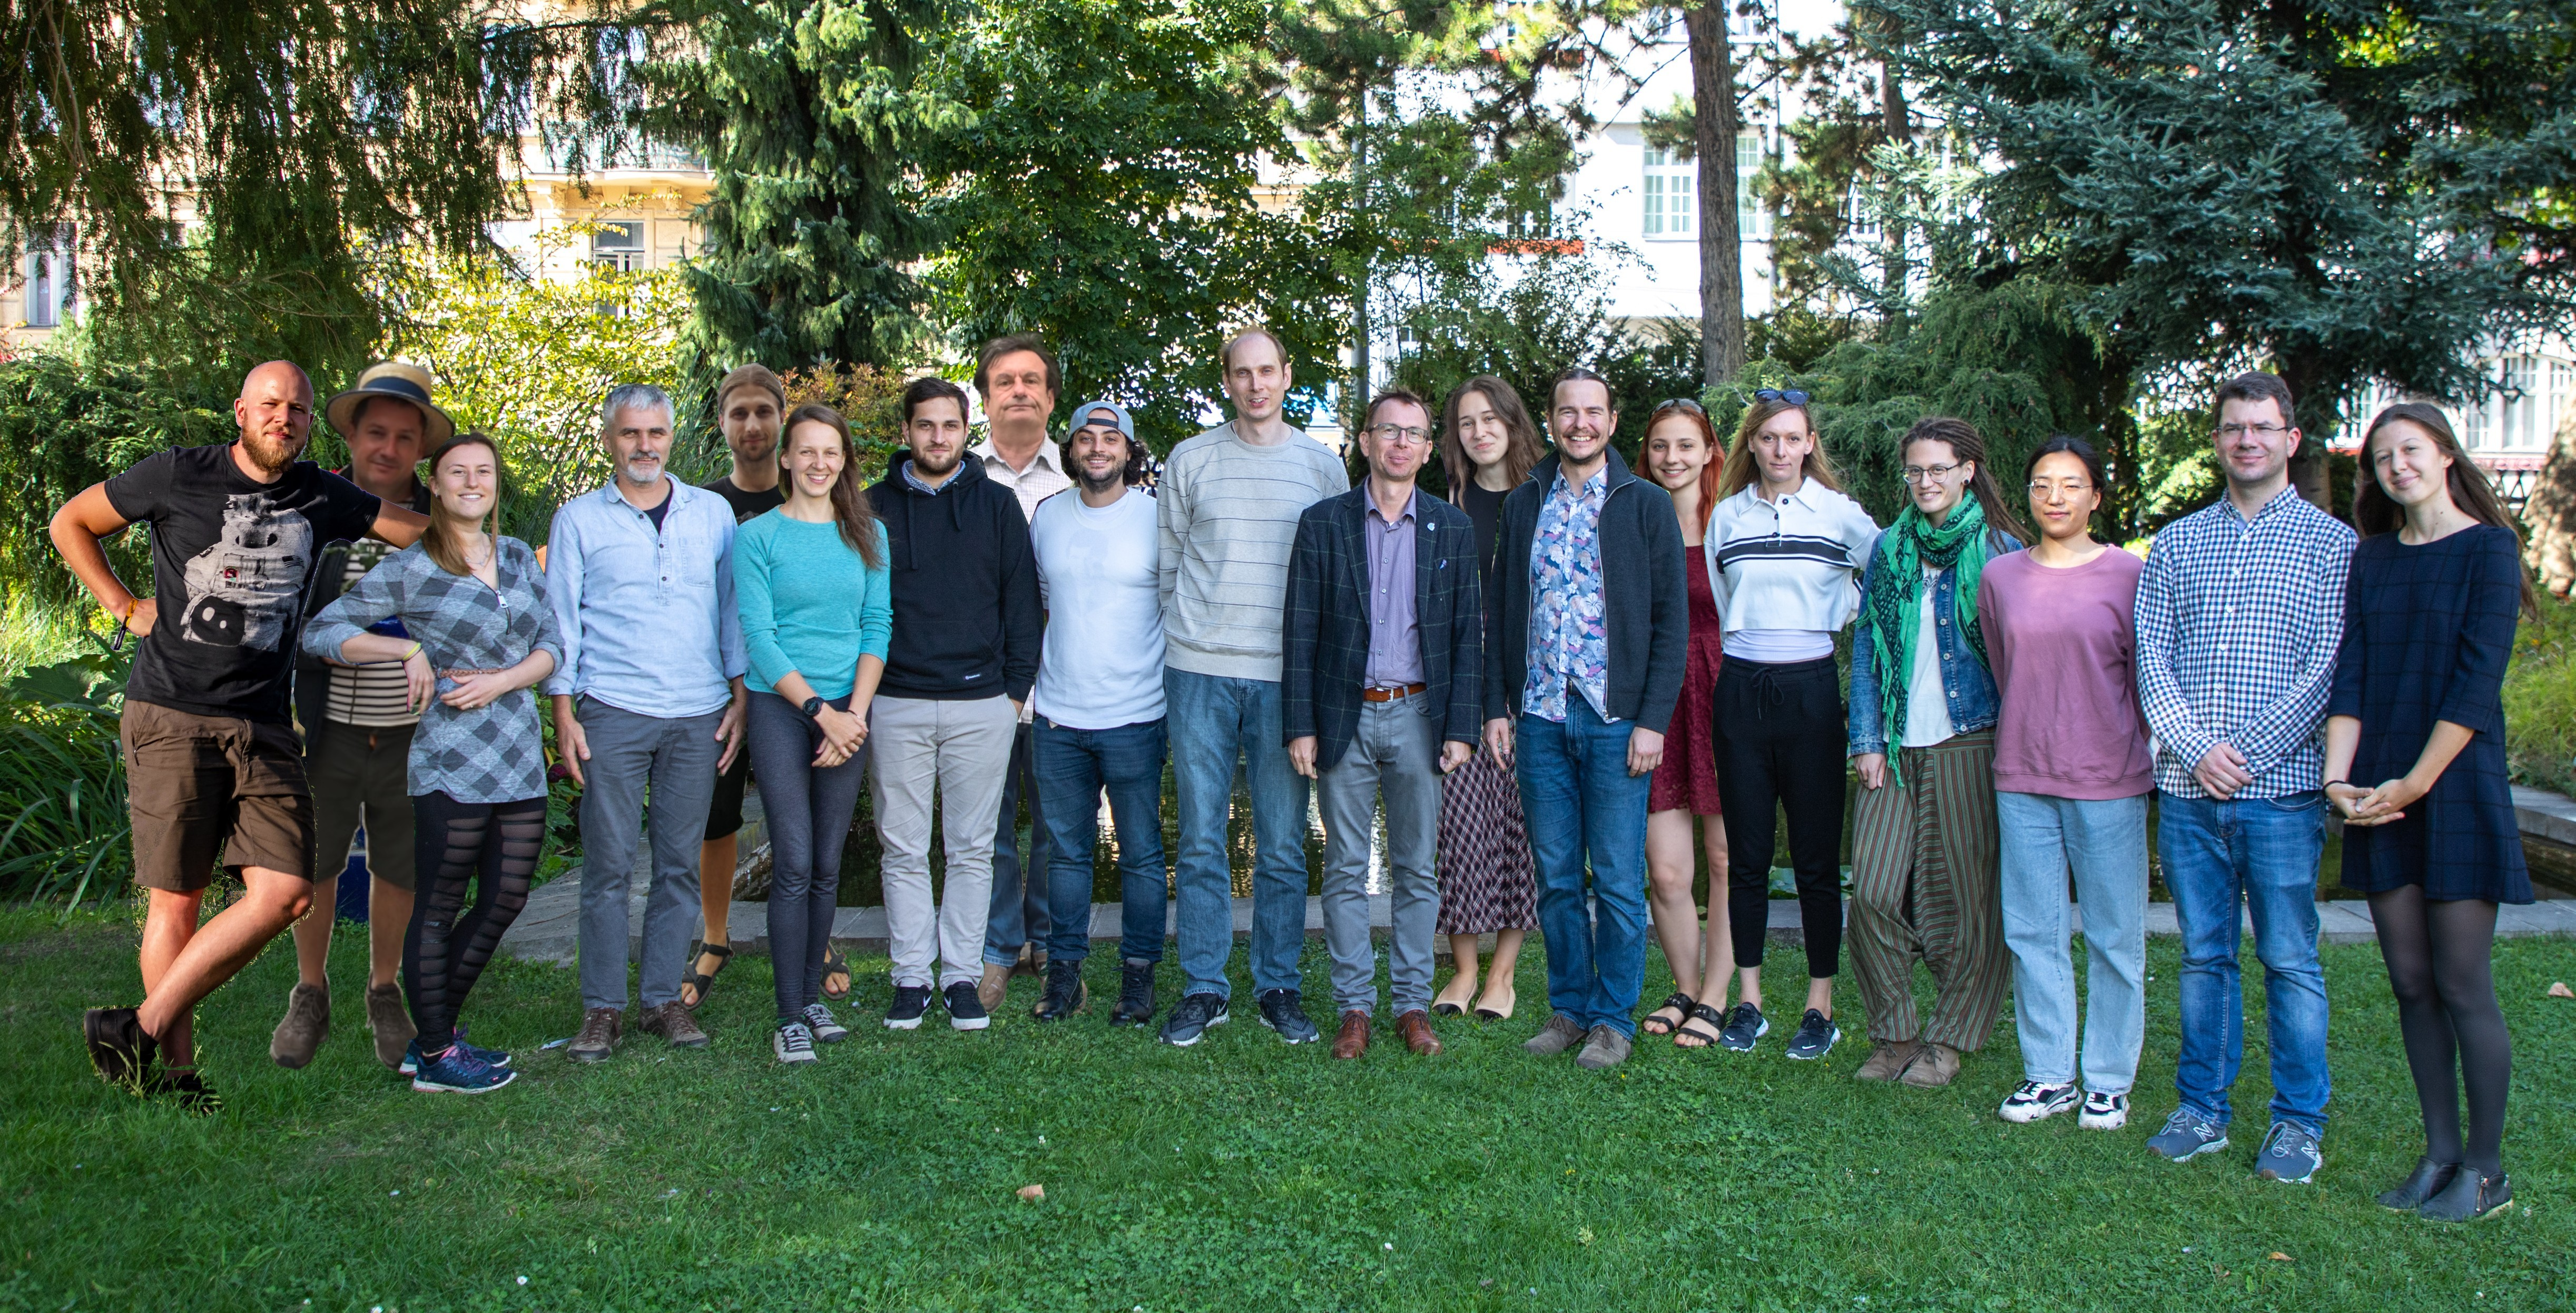
\includegraphics[height=180pt]{HEA/team.jpg}};

    % \draw<2-8> (5.7, 7.55) node {\url{hea.physics.muni.cz}};
    % \draw<2-8> (10.3, 7.0) node {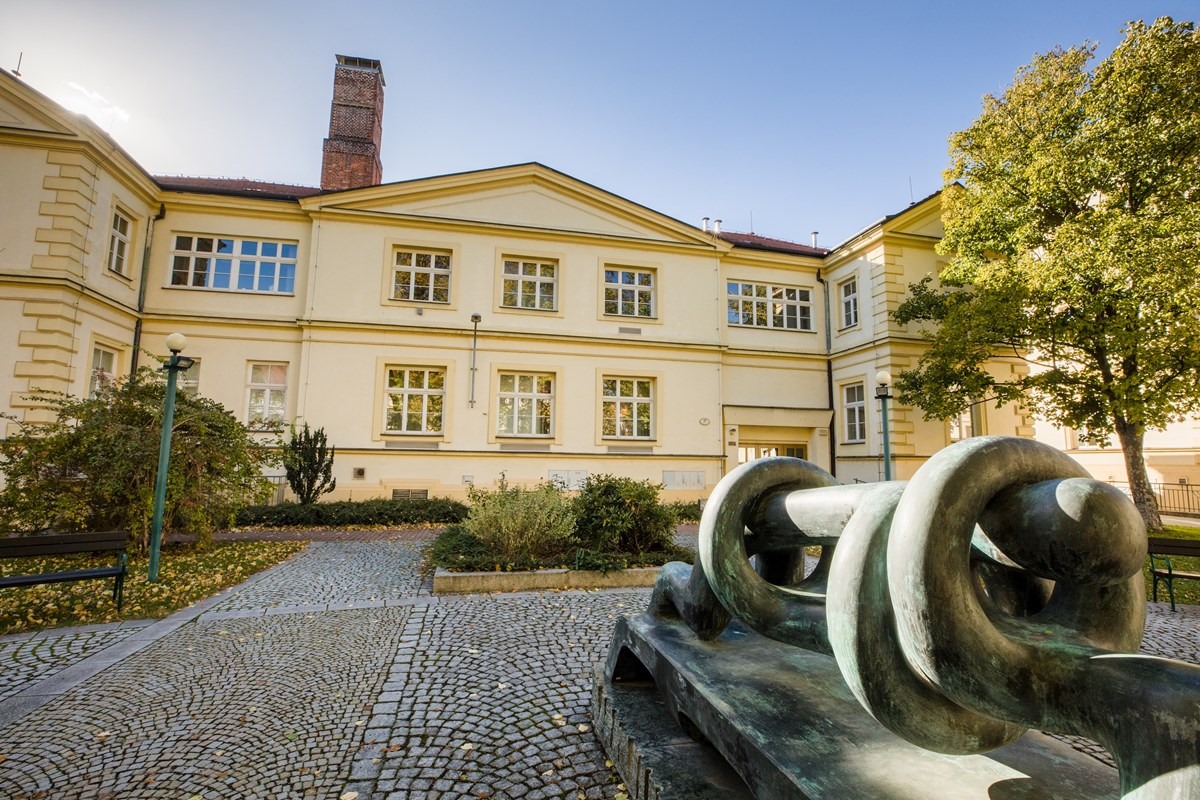
\includegraphics[height=45pt]{HEA/kotlarska.jpg}};
    % \draw<3-8> (10.3, 4.95) node {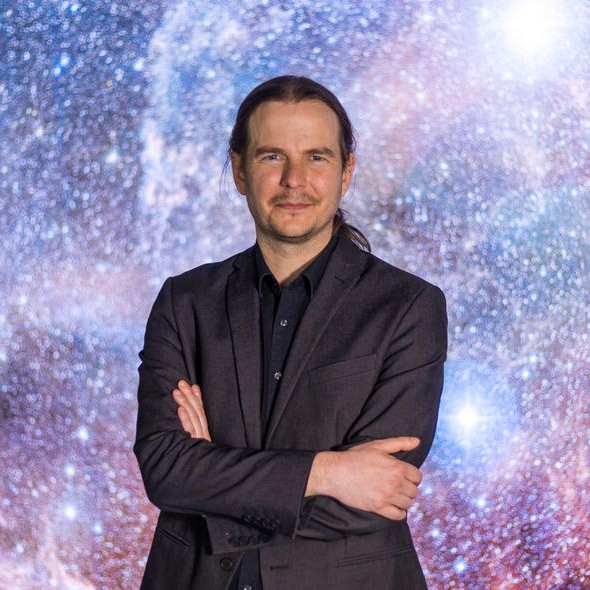
\includegraphics[height=56pt]{HEA/norbert.jpg}};
    % \draw<5-8> (7.34, 3.25) node {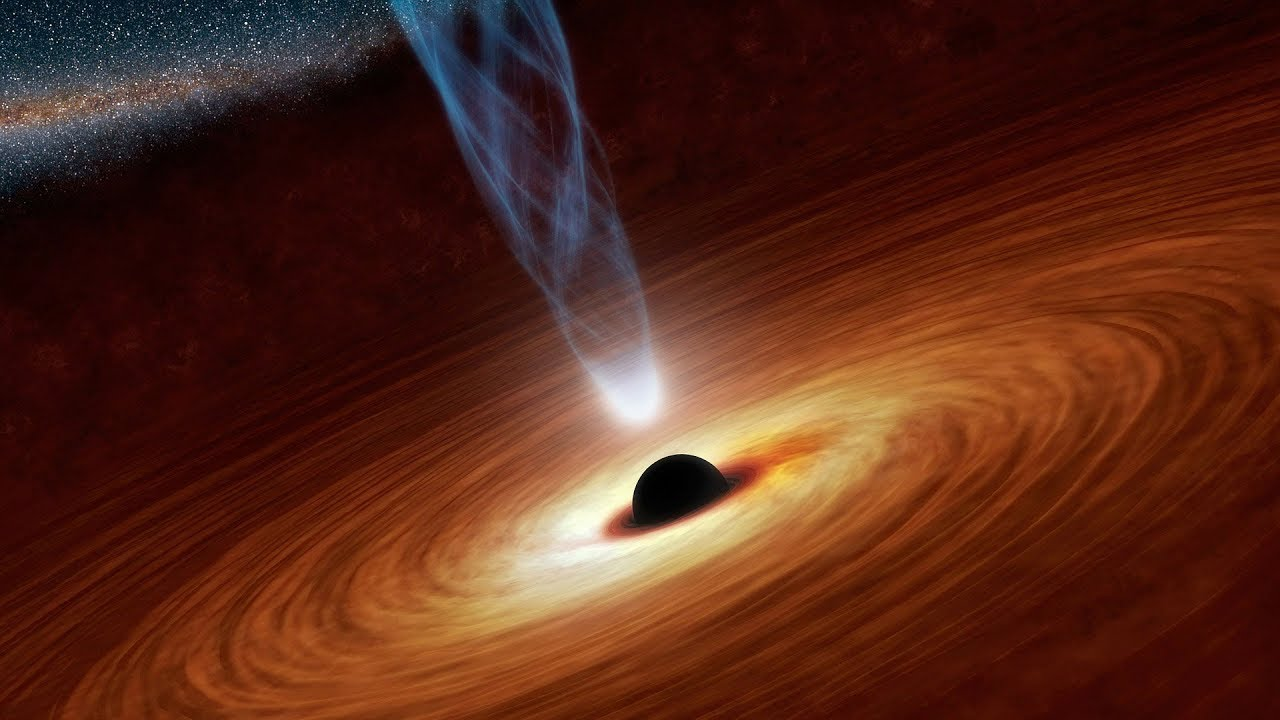
\includegraphics[height=45pt]{HEA/hea.jpg}};
    % \draw<6-8> (9.9, 2.7) node {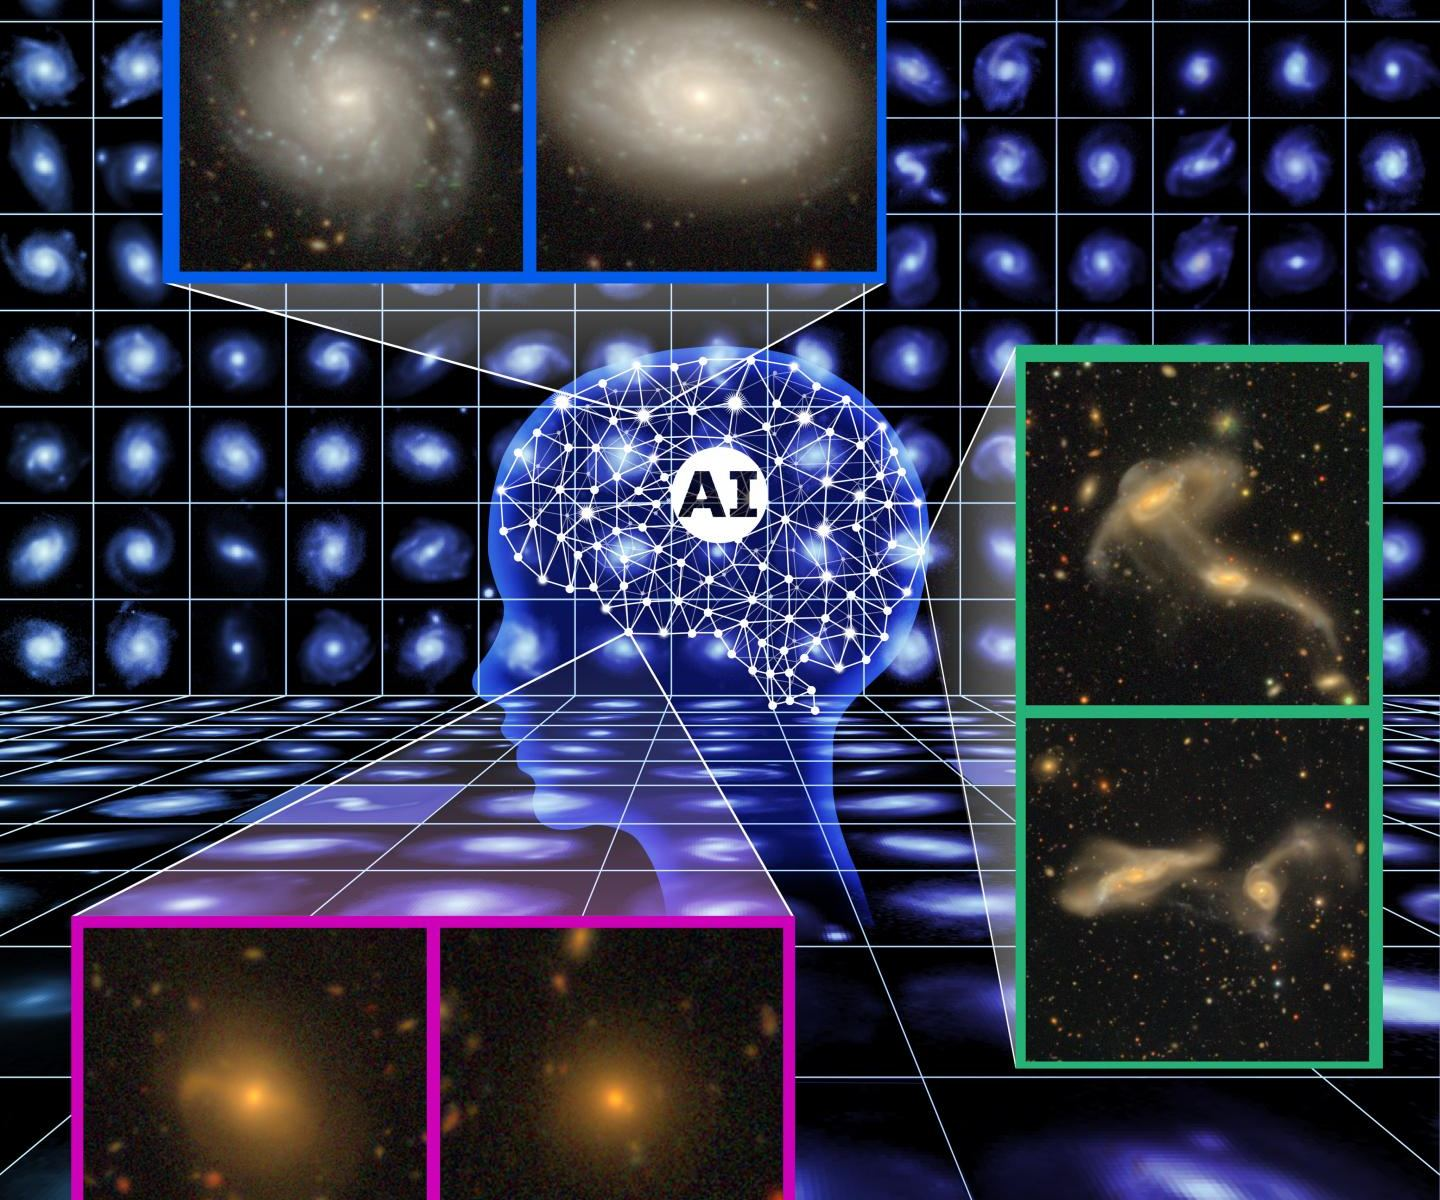
\includegraphics[height=45pt]{HEA/astro_AI.jpg}};
    % \draw<7-8> (7.9, 1.45) node {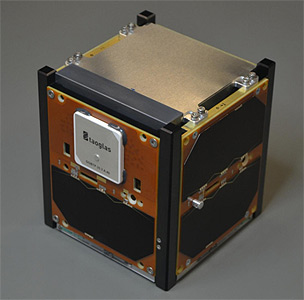
\includegraphics[height=45pt]{HEA/grbalpha.jpg}};
    % \draw<8> (9.75, 0.9) node {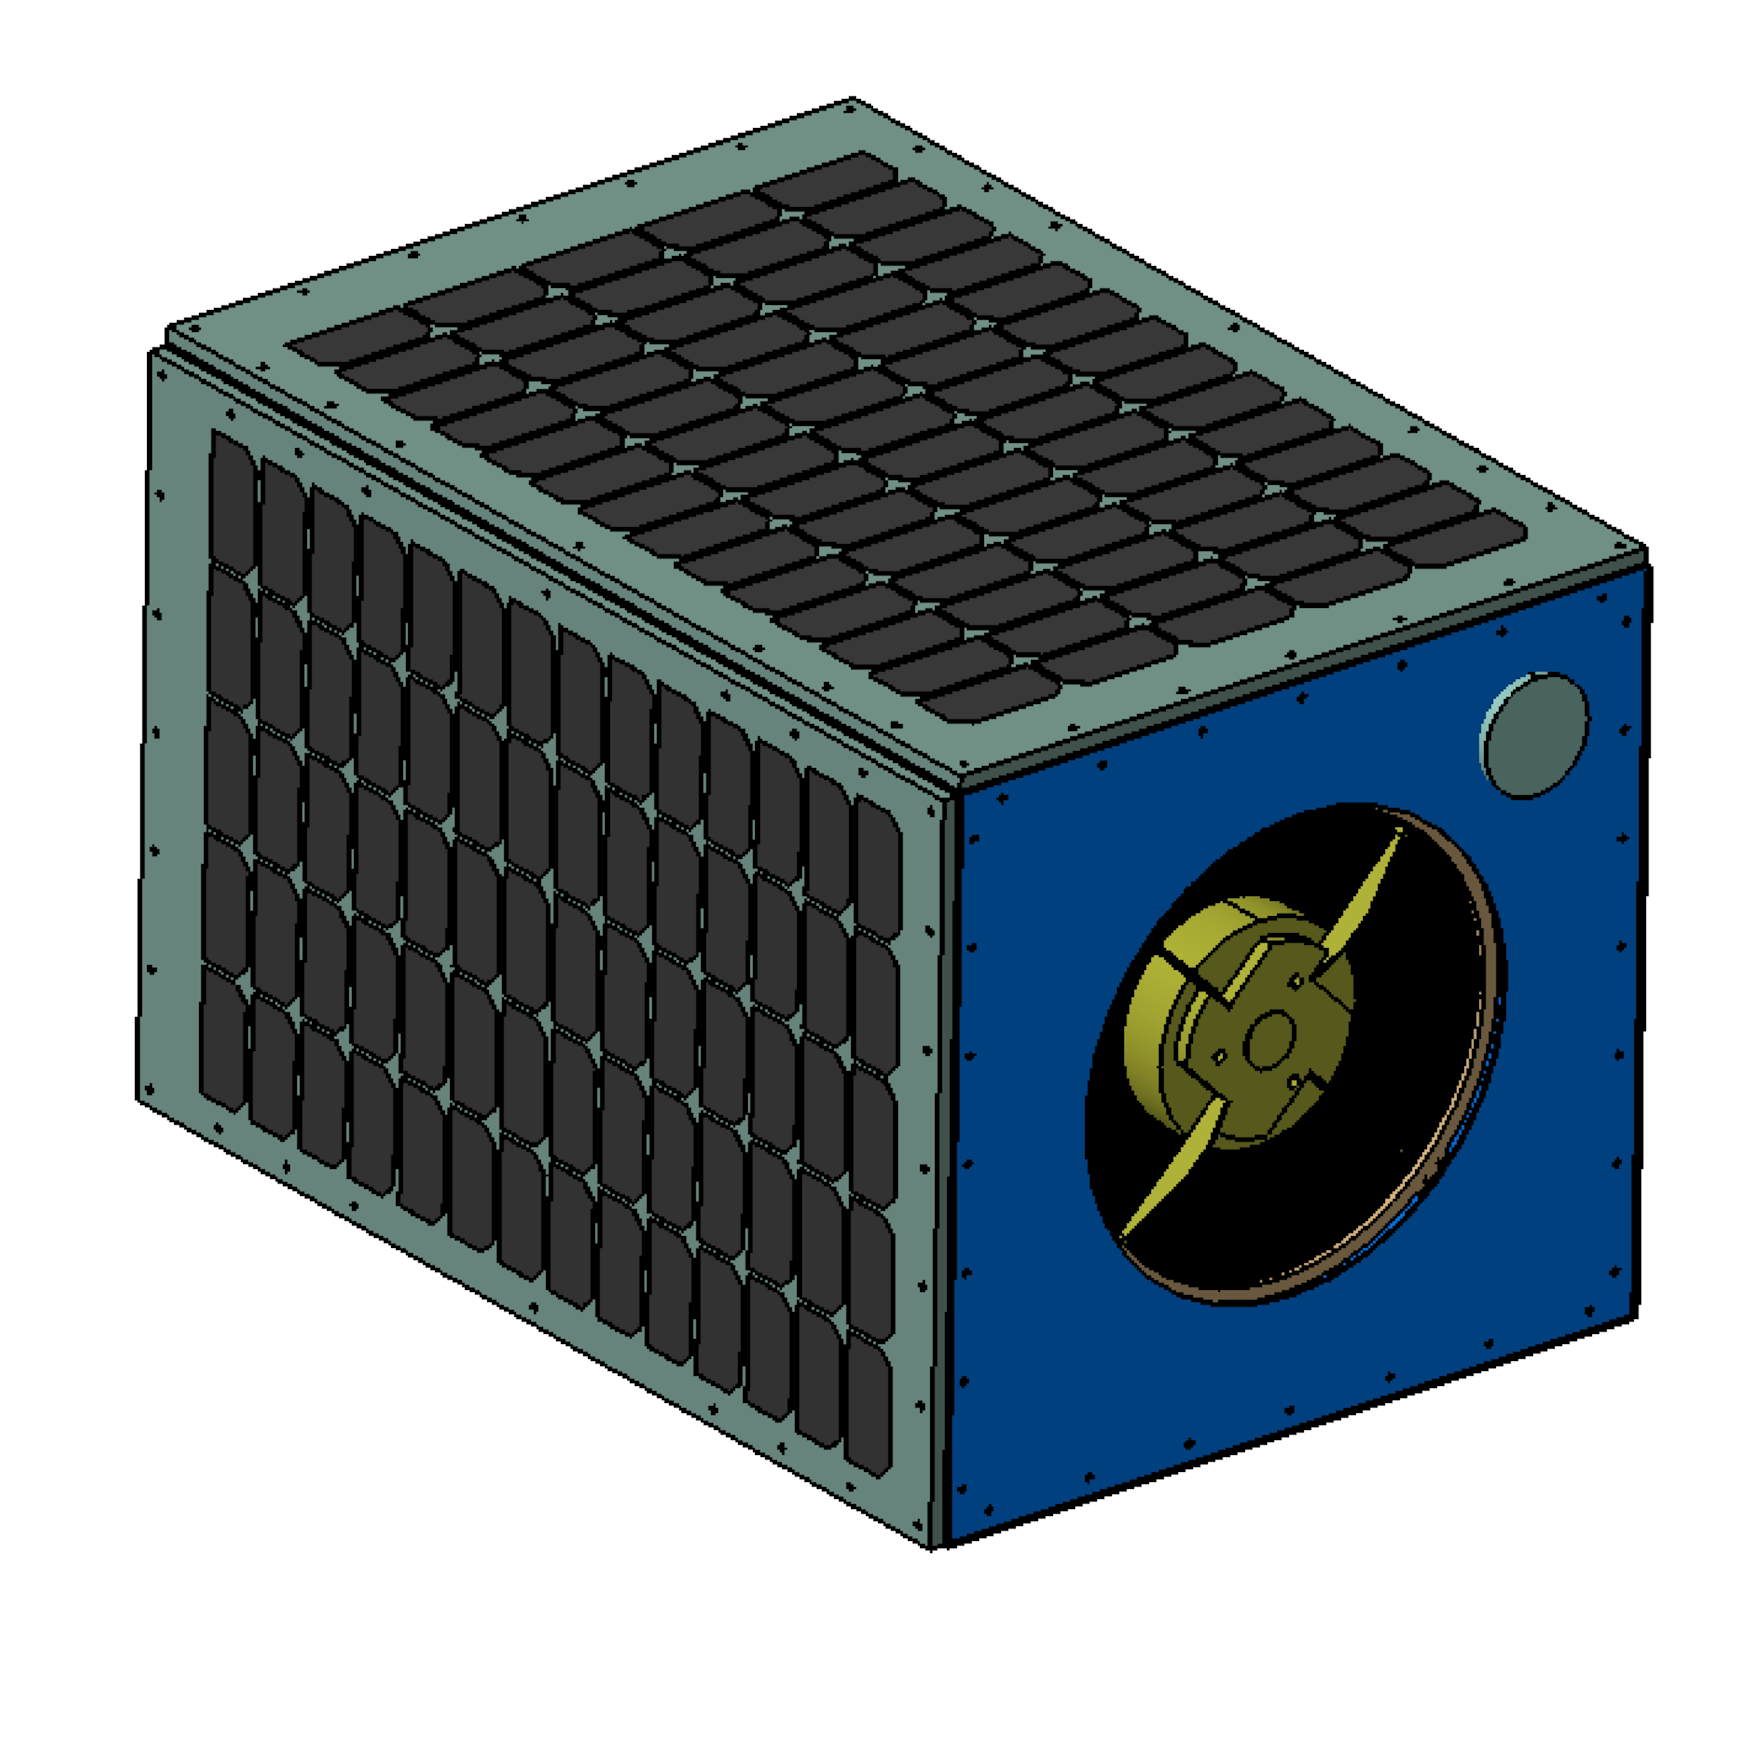
\includegraphics[height=45pt]{HEA/quvik.png}};

    \draw<1> (5.7, 4.0) node  {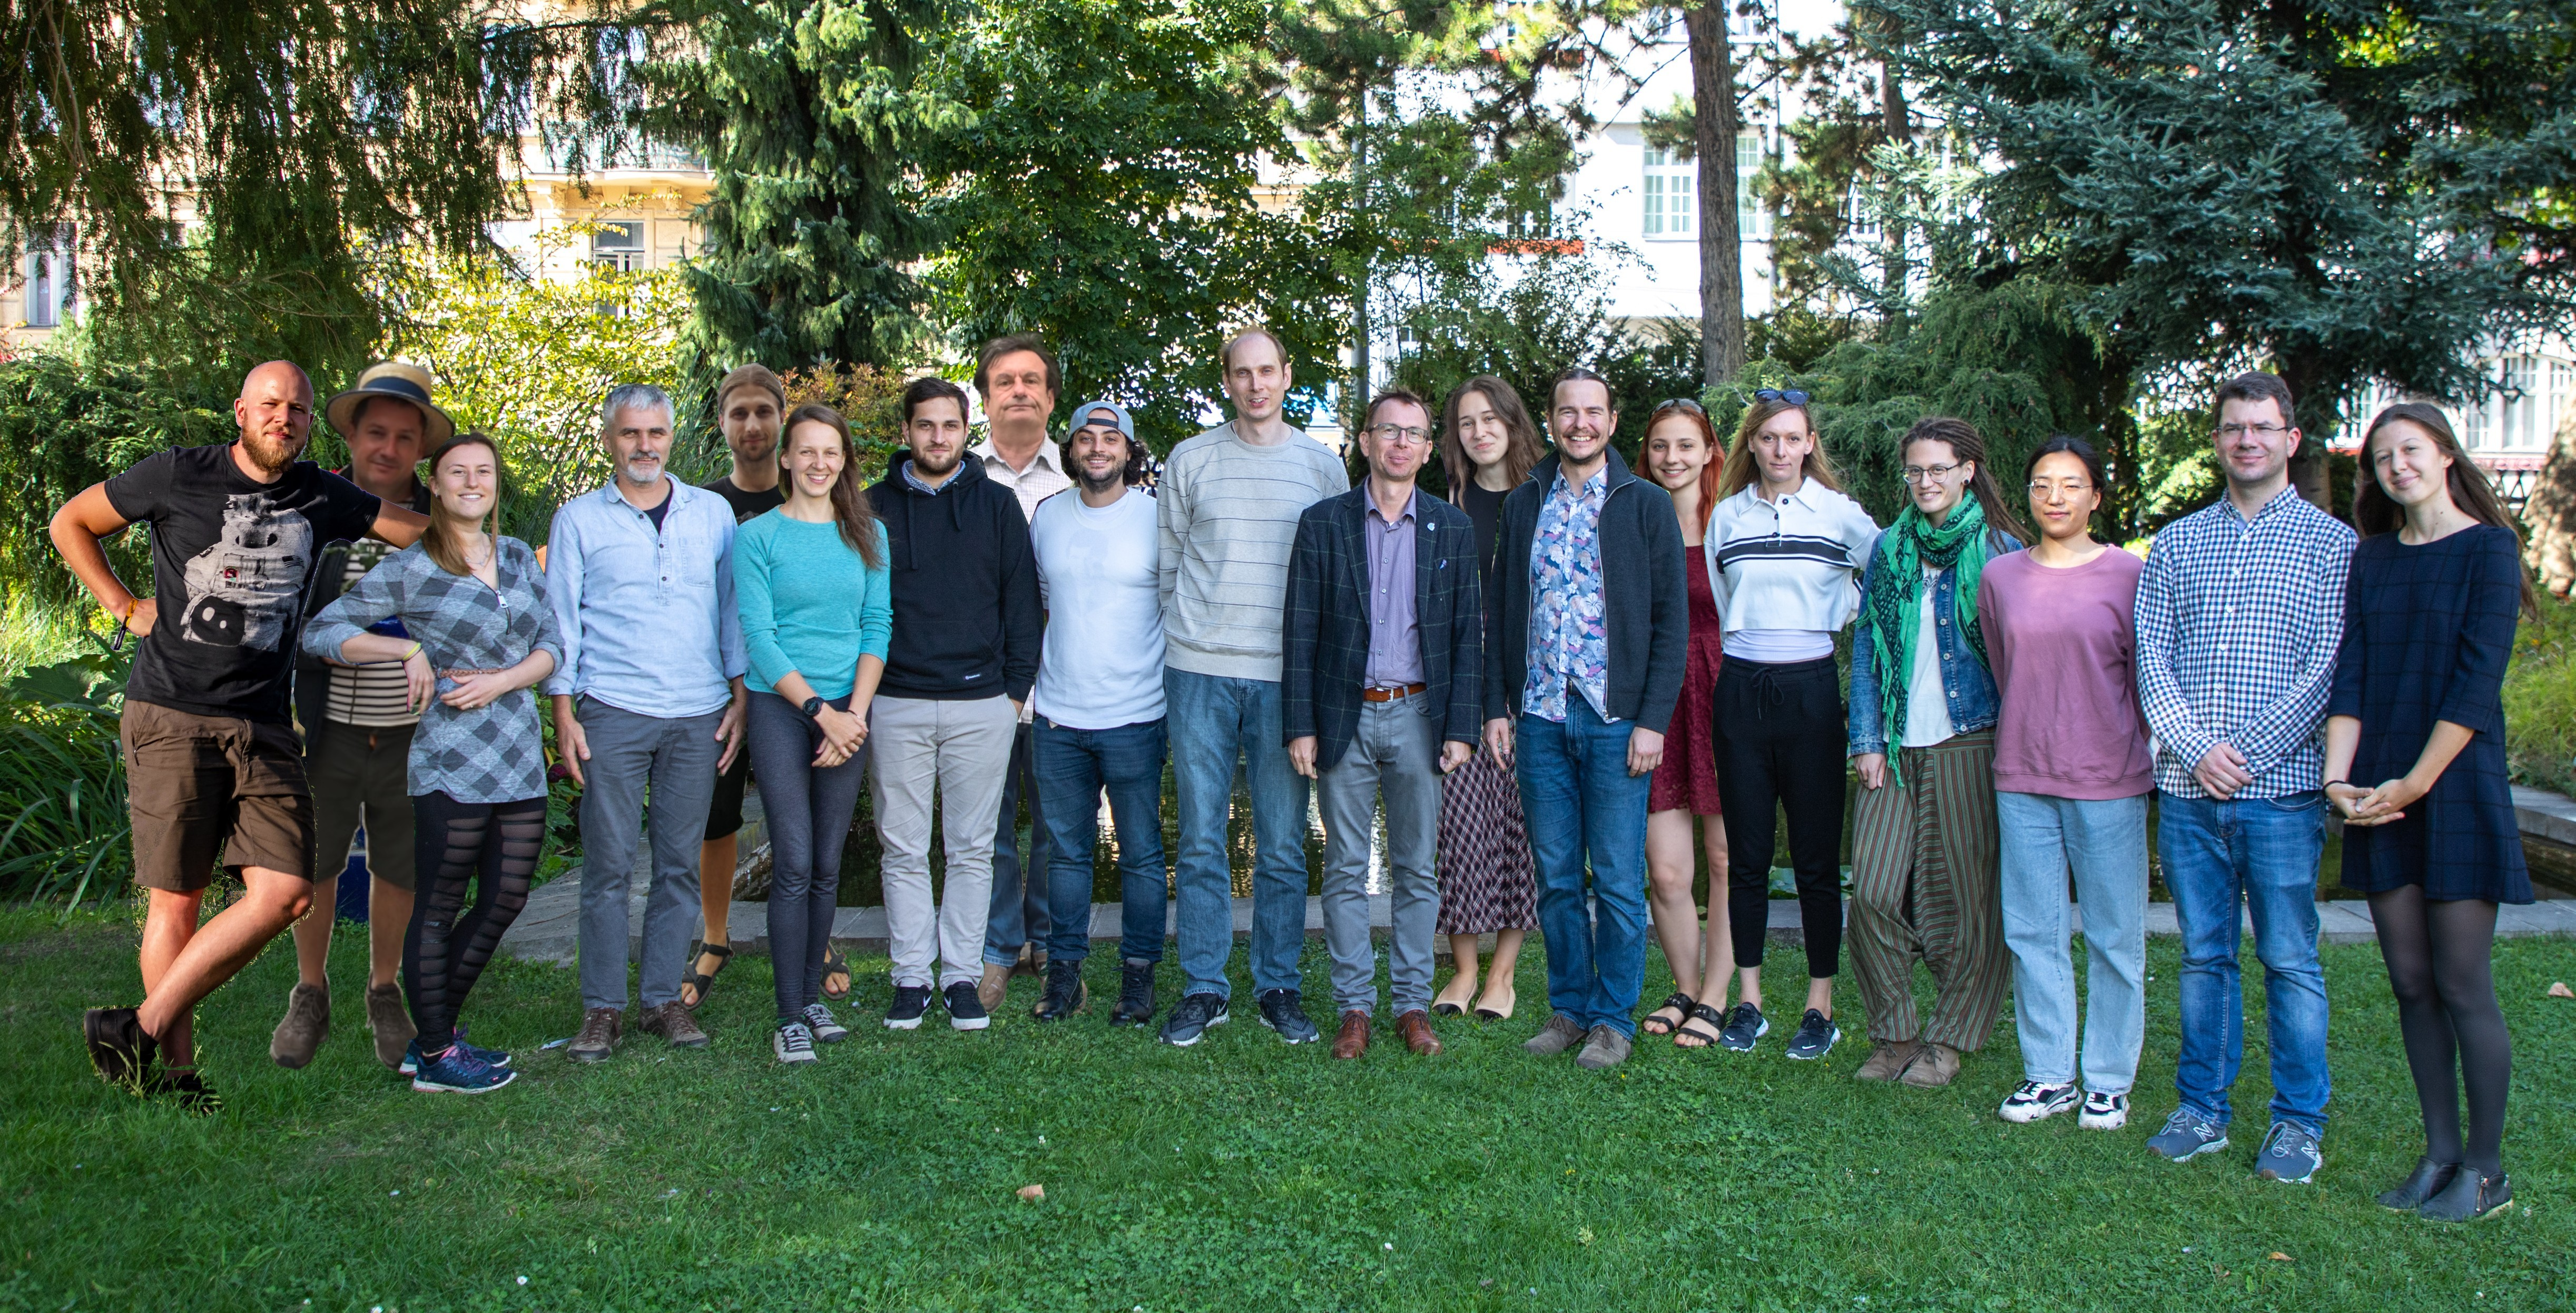
\includegraphics[height=180pt]{HEA/team.jpg}};

    \draw<2> (5.7, 7.15) node {\url{www.hea.physics.muni.cz}};
    \draw<2> (10.0, 6.70) node {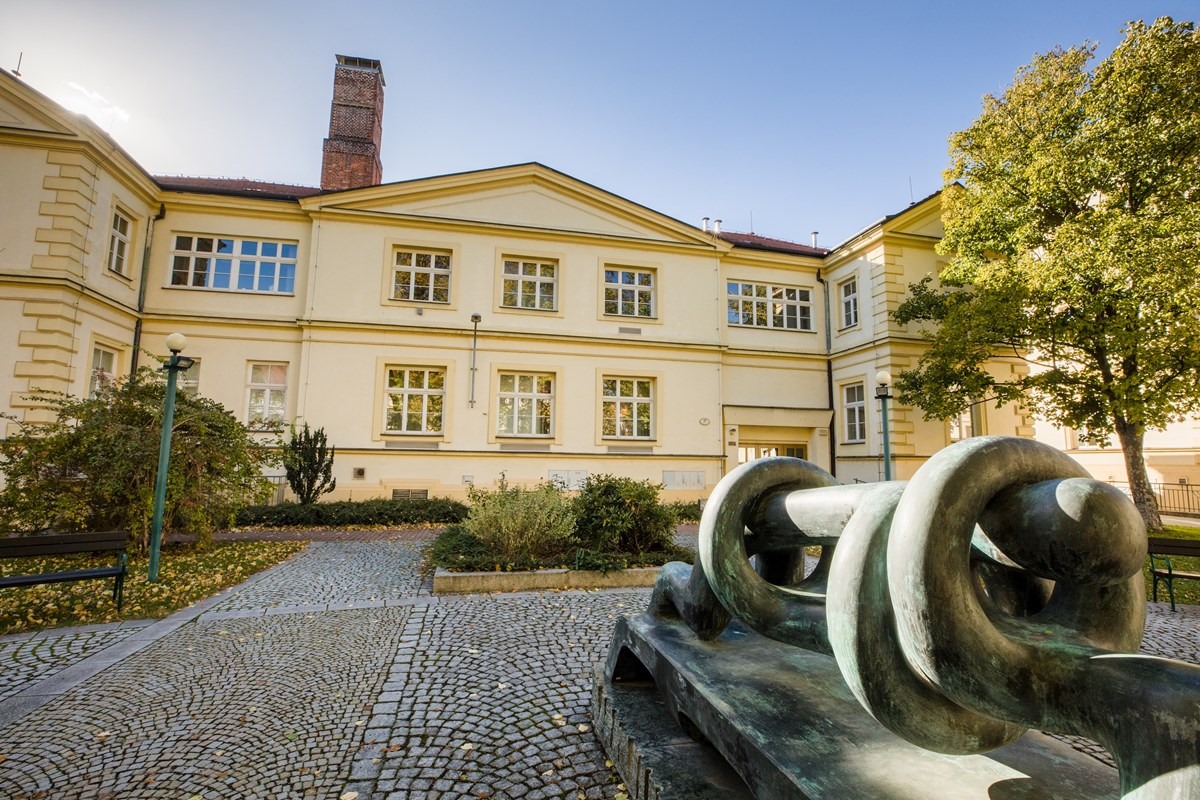
\includegraphics[height=49pt]{HEA/kotlarska.jpg}};
    \draw<2> (10.3, 4.65) node {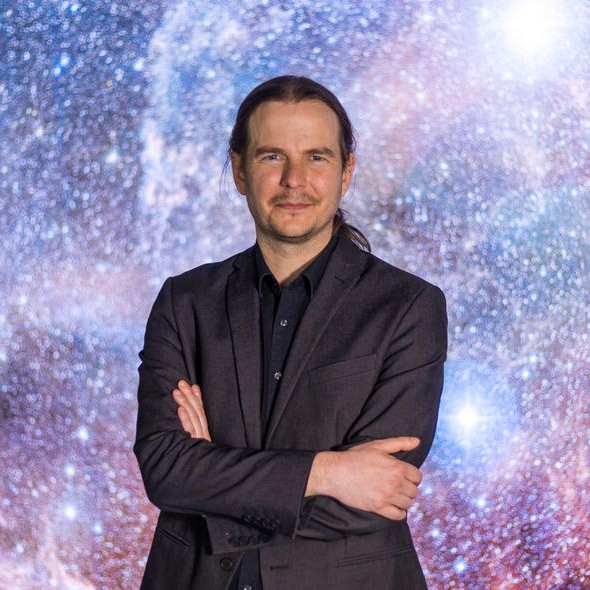
\includegraphics[height=56pt]{HEA/norbert.jpg}};
    \draw<2> (7.34, 3.25) node {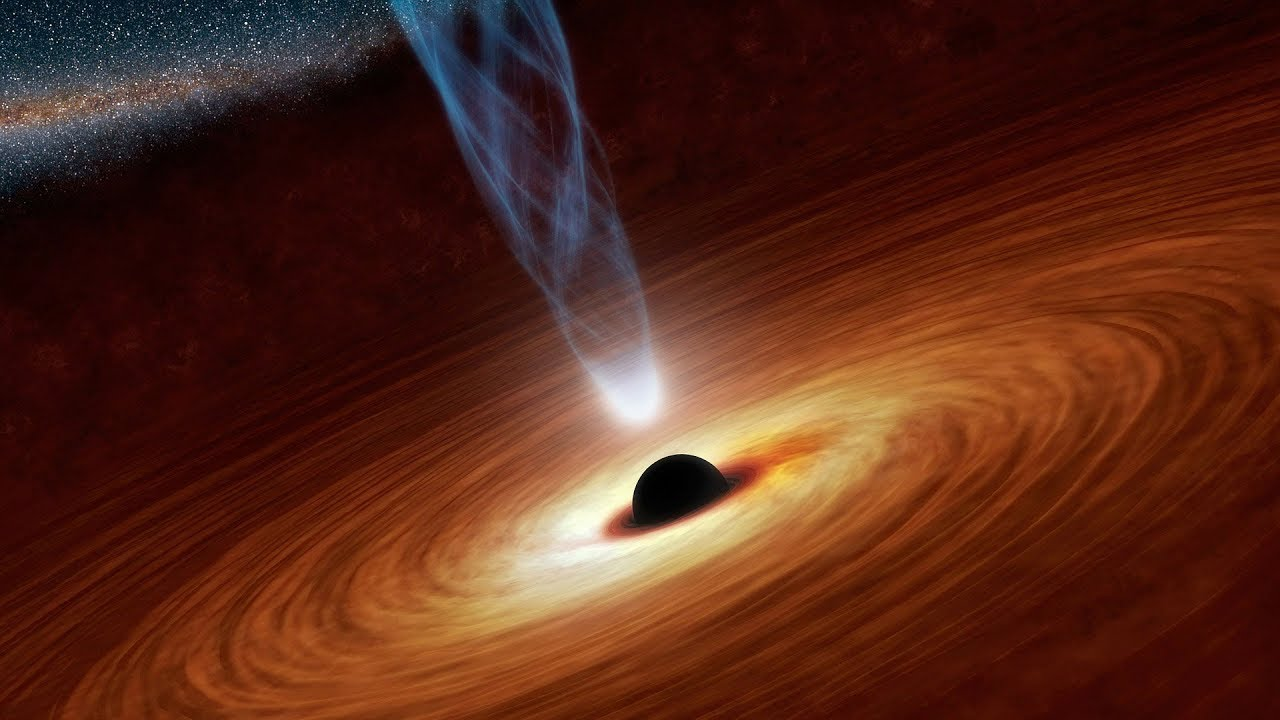
\includegraphics[height=45pt]{HEA/hea.jpg}};
    \draw<2> (10.1, 2.5) node {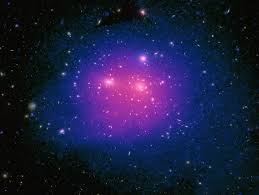
\includegraphics[height=50pt]{HEA/galaxy_cluster.png}};
    \draw<2> (7.9, 1.25) node {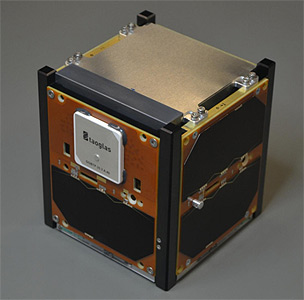
\includegraphics[height=45pt]{HEA/grbalpha.jpg}};
    \draw<2> (9.75, 0.7) node {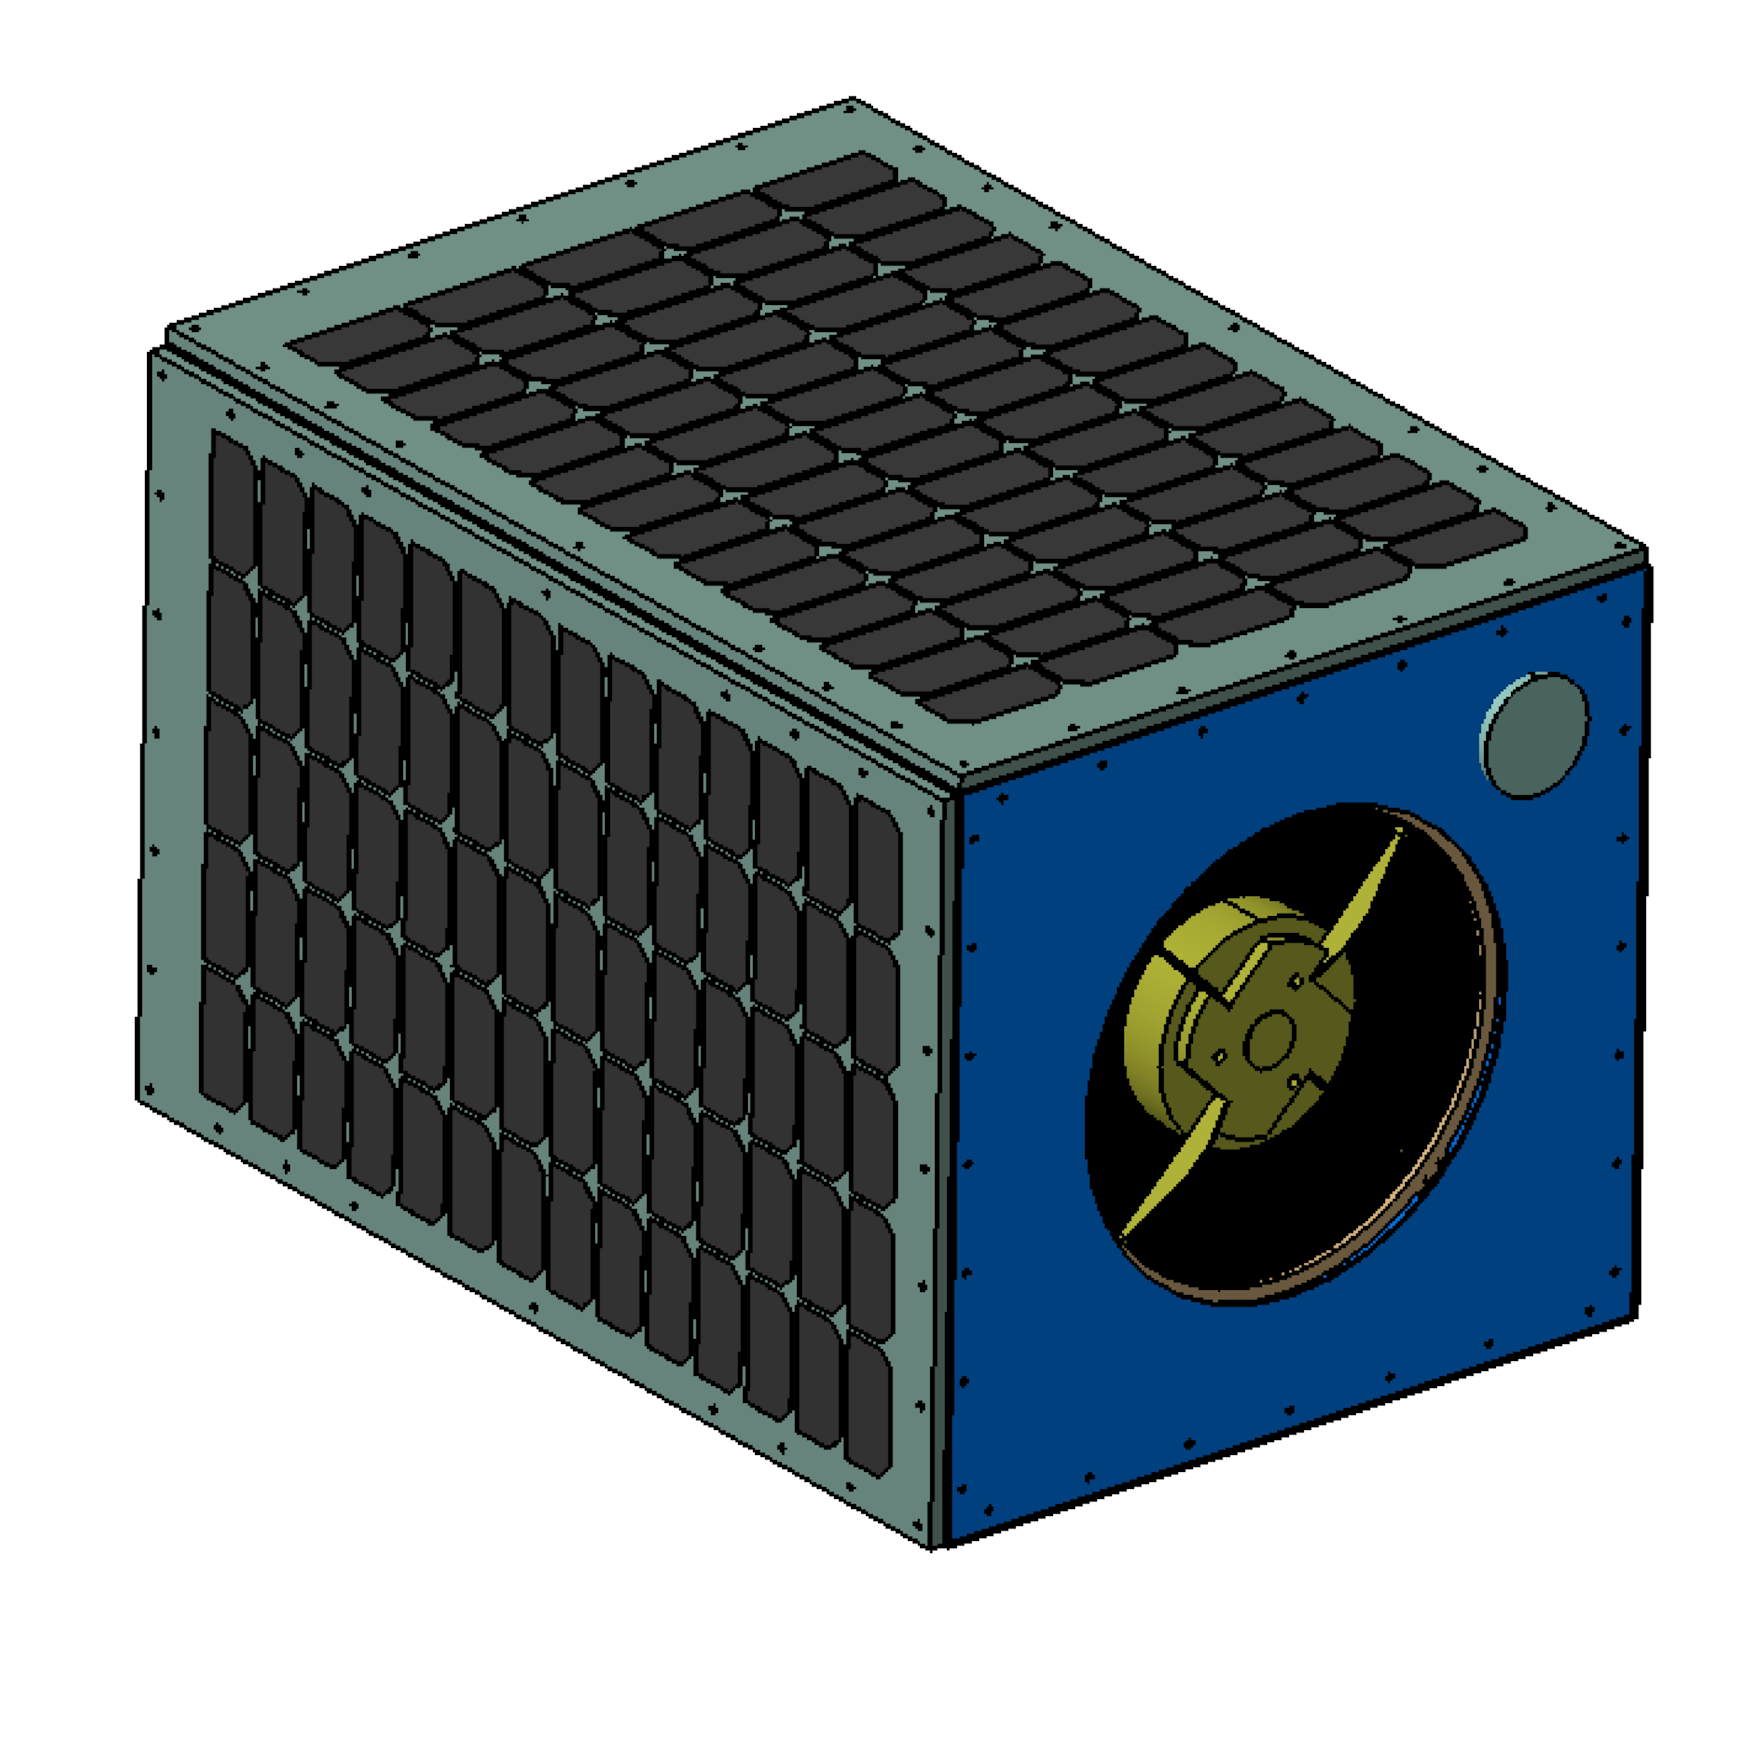
\includegraphics[height=45pt]{HEA/quvik.png}};
\end{tikzpicture}
\end{frame}


\begin{frame}{\vs Obsah \lend}
\vspace{5mm}
\begin{itemize}
    \item<alert@1> Umělá inteligence\\ \vspace{7mm}
    \item<alert@2> Neuronová síť\\ \vspace{7mm}
    \item<alert@3> Využití umělé inteligence\\ \vspace{7mm}
    \item<alert@4> Umělá inteligence v astronomii\\ \vspace{7mm}
    \item<alert@5> Cavity Detection Tool (CADET)
\end{itemize}
\begin{tikzpicture}[remember picture,overlay,shift={(current page.center)}]
    \draw<1-> (0.4, 1.4) node {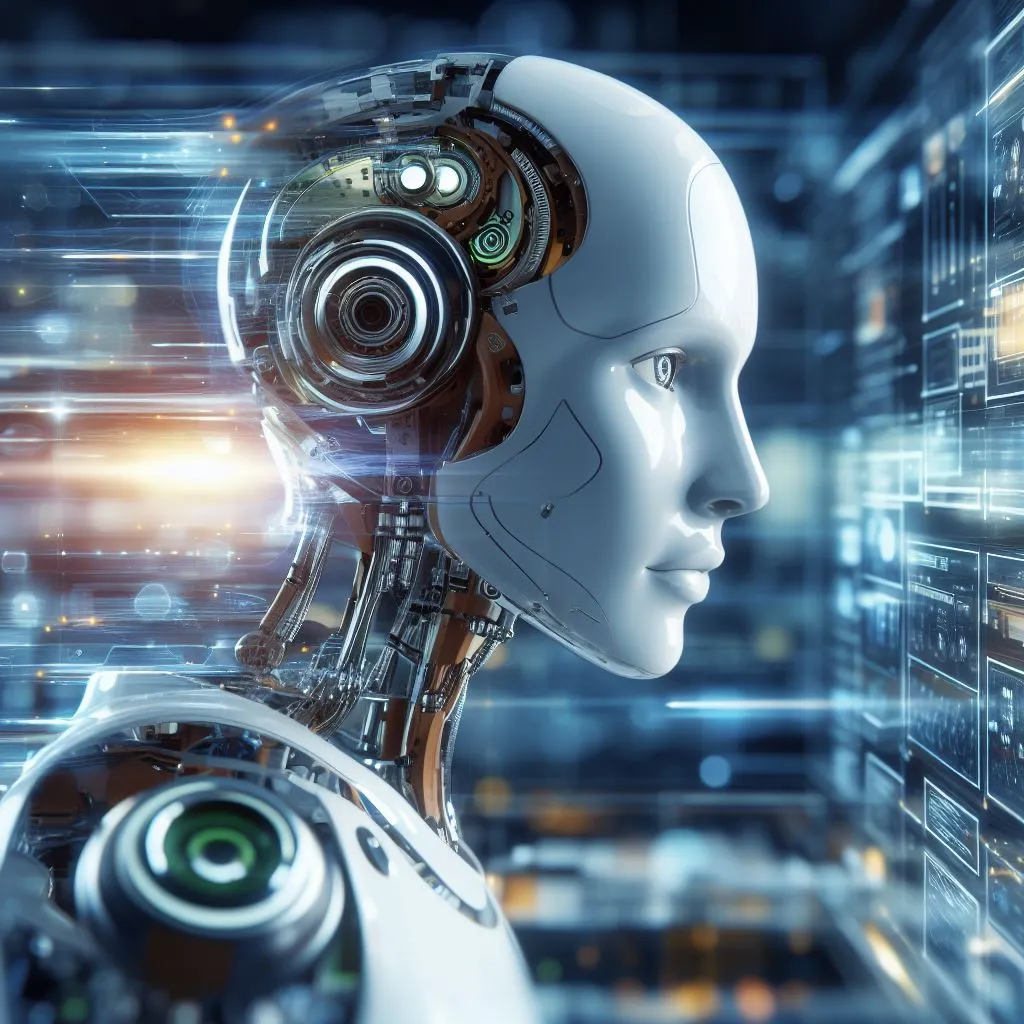
\includegraphics[height=50pt]{AI/agi.png}};
    \draw<2-> (3.7, 0.4) node {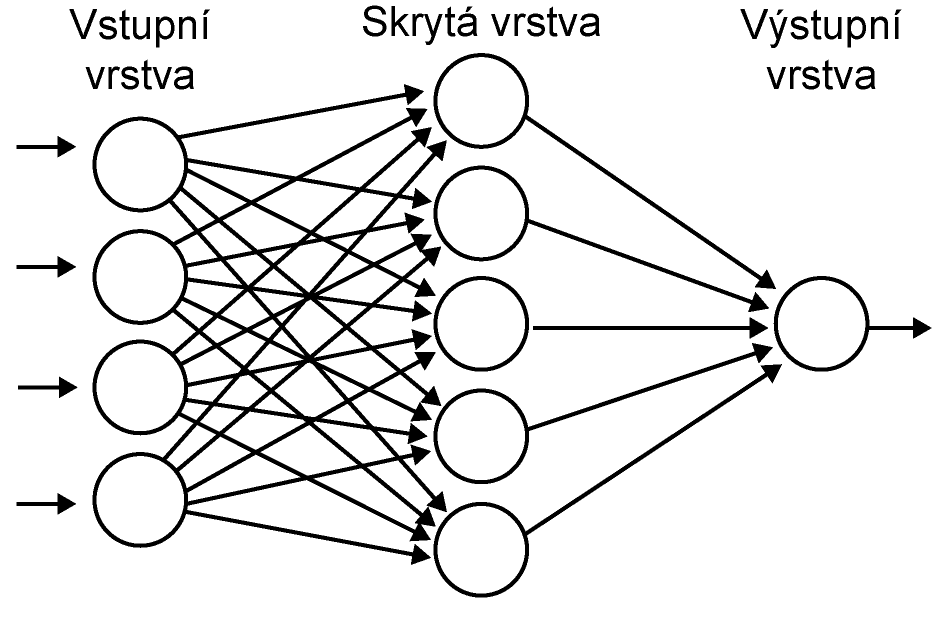
\includegraphics[height=50pt]{AI/neuronova_sit.png}};
    \draw<3-> (0.9, -0.7) node {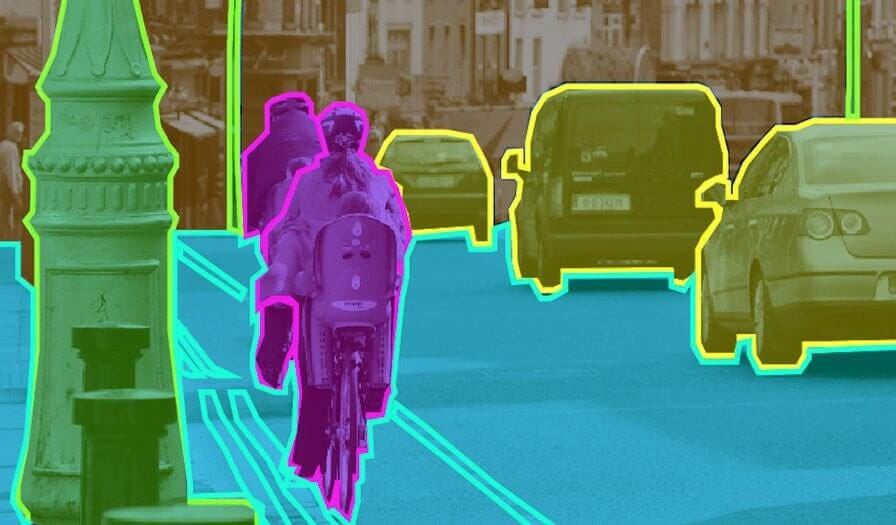
\includegraphics[height=40pt]{AI/segmentation.jpg}};
    \draw<4-> (3.9, -1.9) node {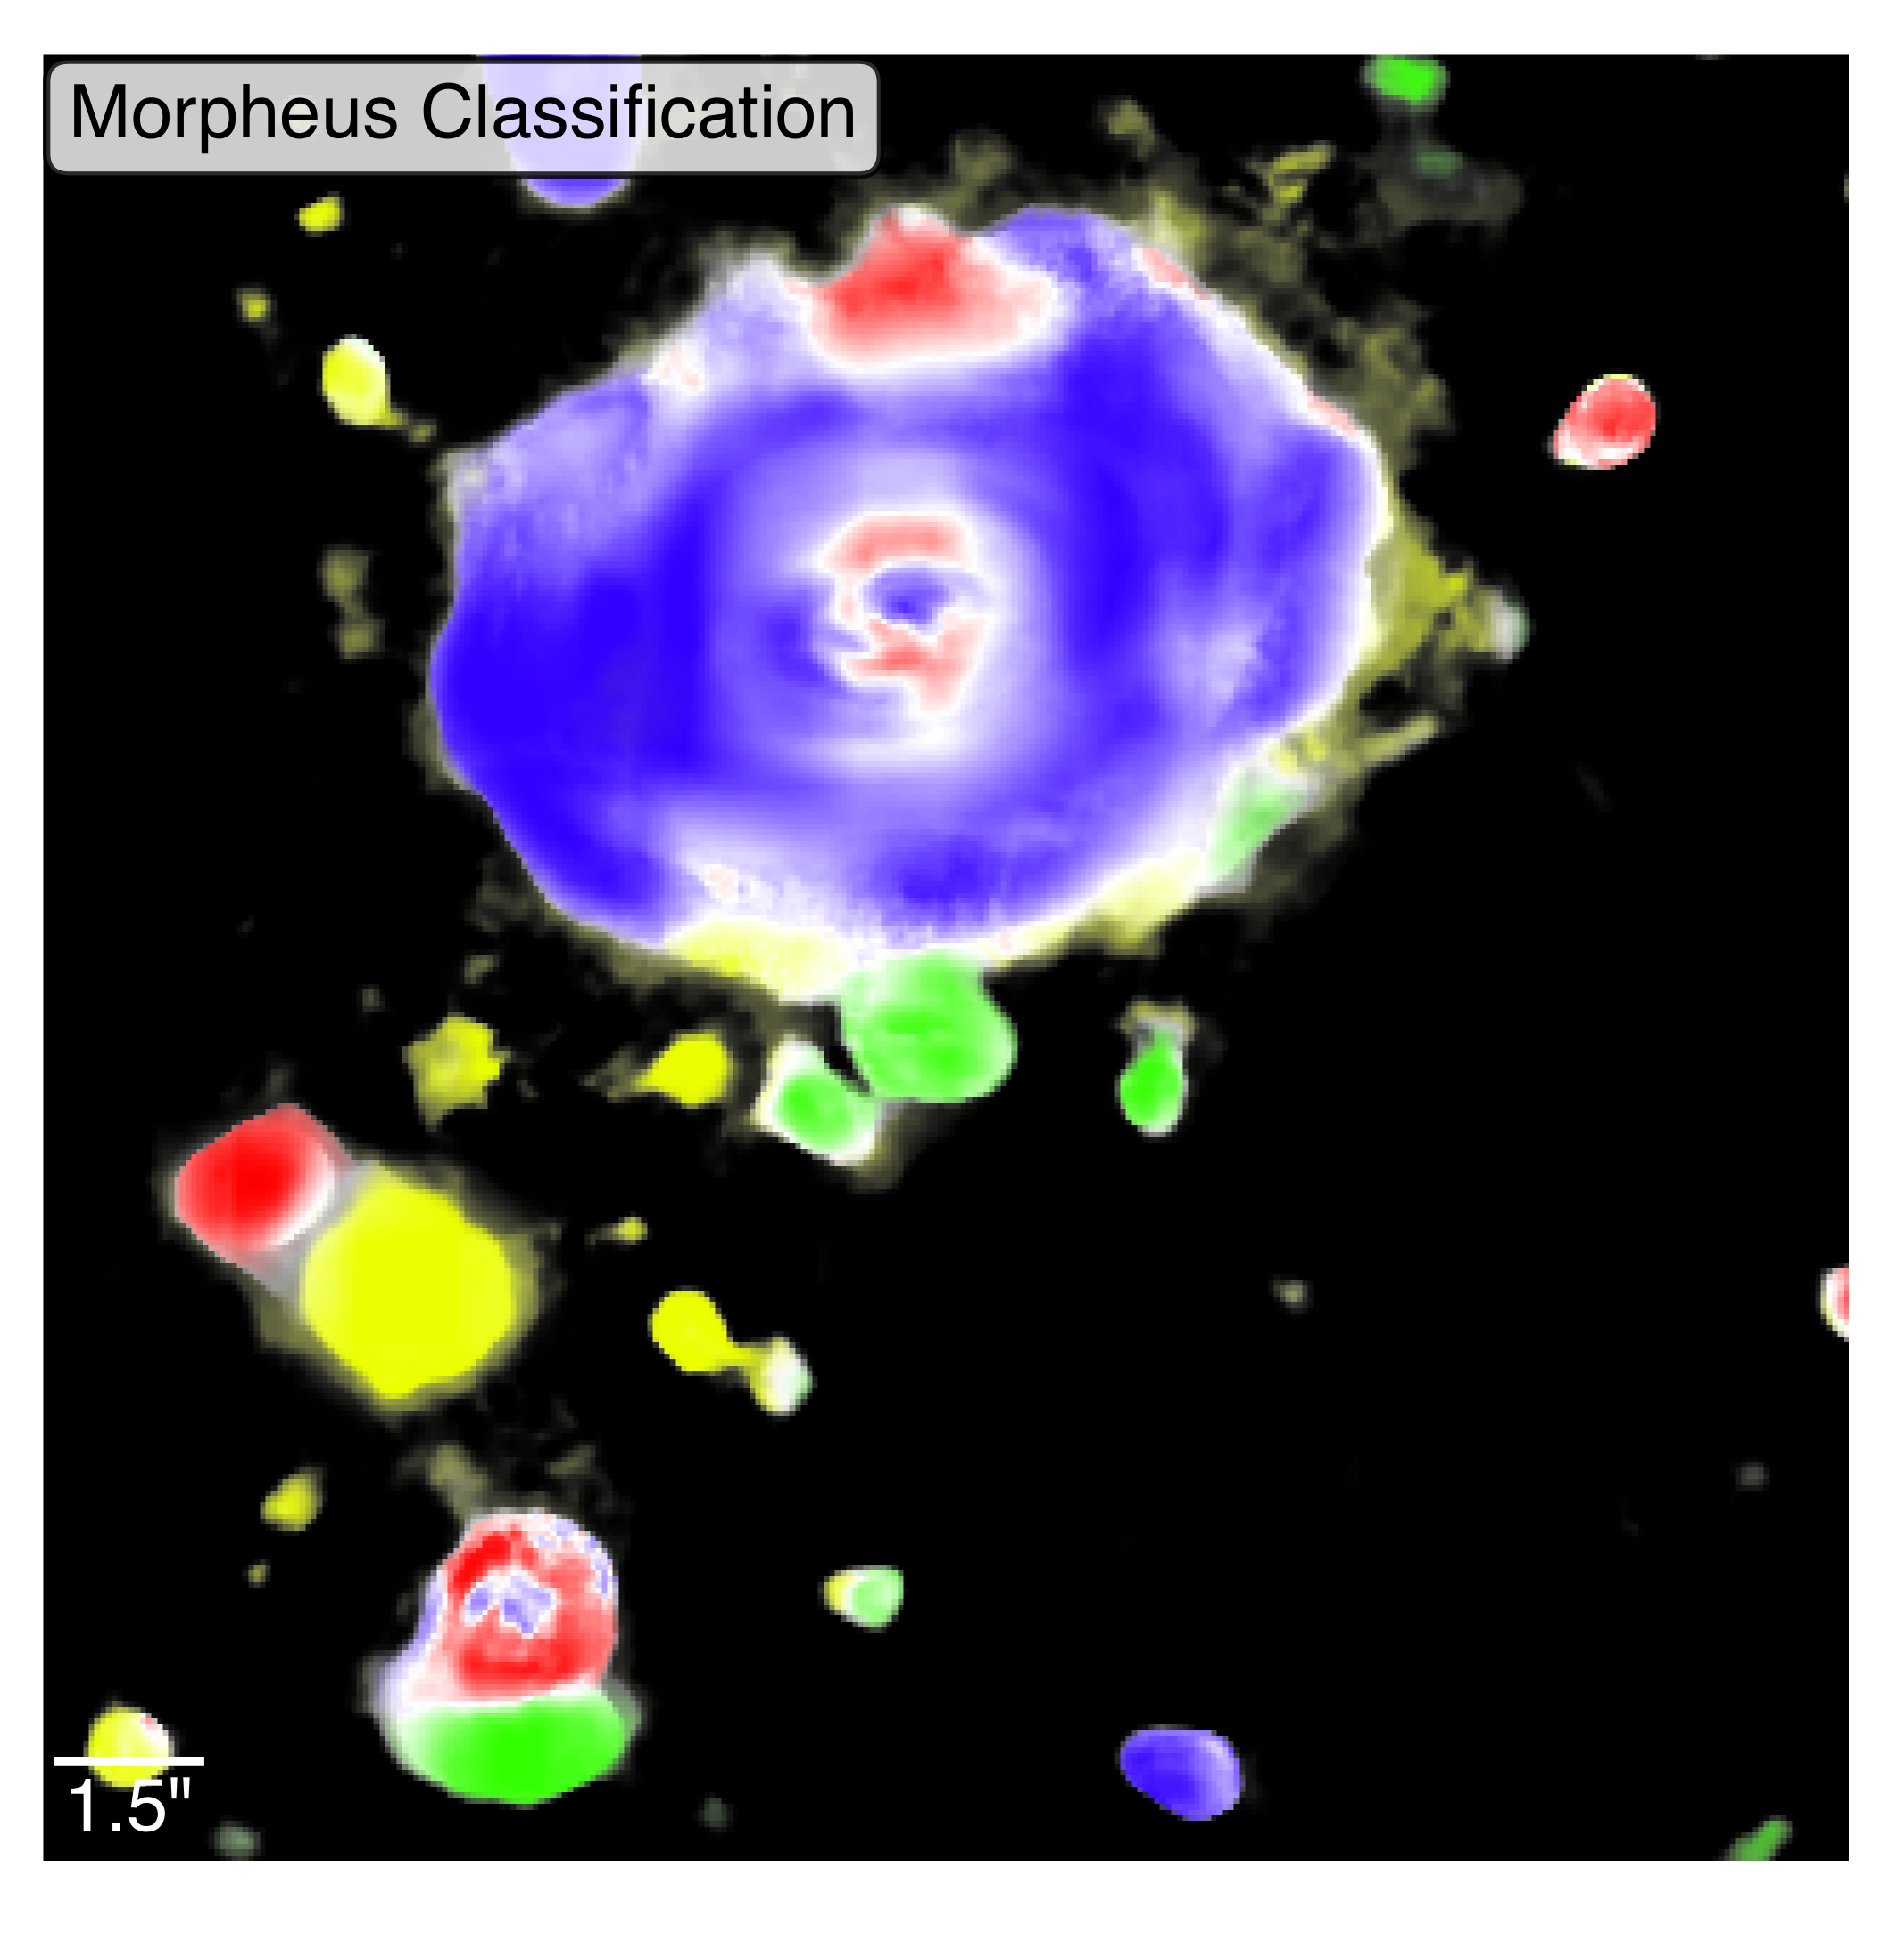
\includegraphics[height=53pt]{AI/morpheus_cut.png}};
    \draw<5-> (1.4, -3.3) node {
\includegraphics[height=50pt]{CADET/CADET.png}};
\end{tikzpicture}
\end{frame}


\section{Umělá inteligence}

\begin{frame}{\vs Co je to AI? \lend}
\begin{tikzpicture}[remember picture,overlay,shift={(current page.center)}]
    \draw<1-> (3.2, 0.55) node {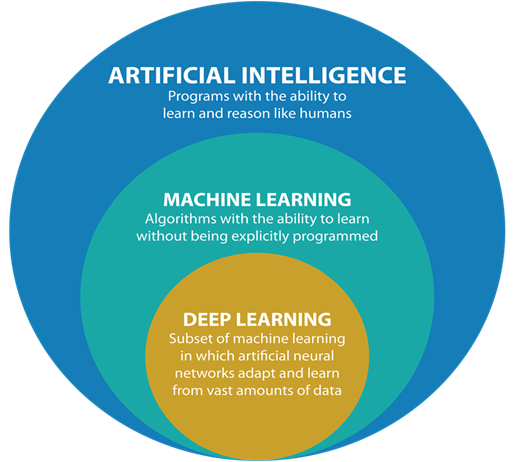
\includegraphics[width=155pt]{AI/AI_ML_DL.png}};
    % \draw<2-4> (3.0, -3.0) node {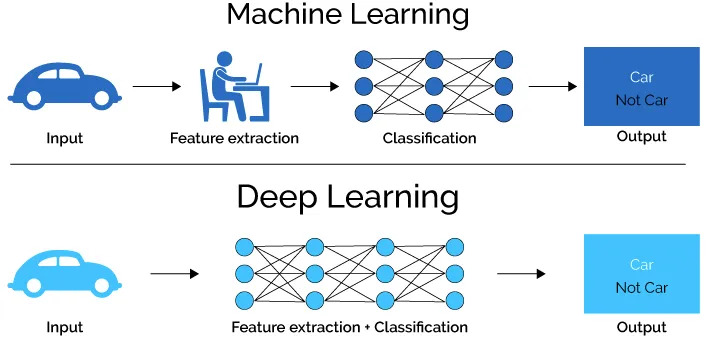
\includegraphics[height=80pt]{AI/ML_vs_DL.jpg}};
    \draw<4> (2.1, -3.3) node {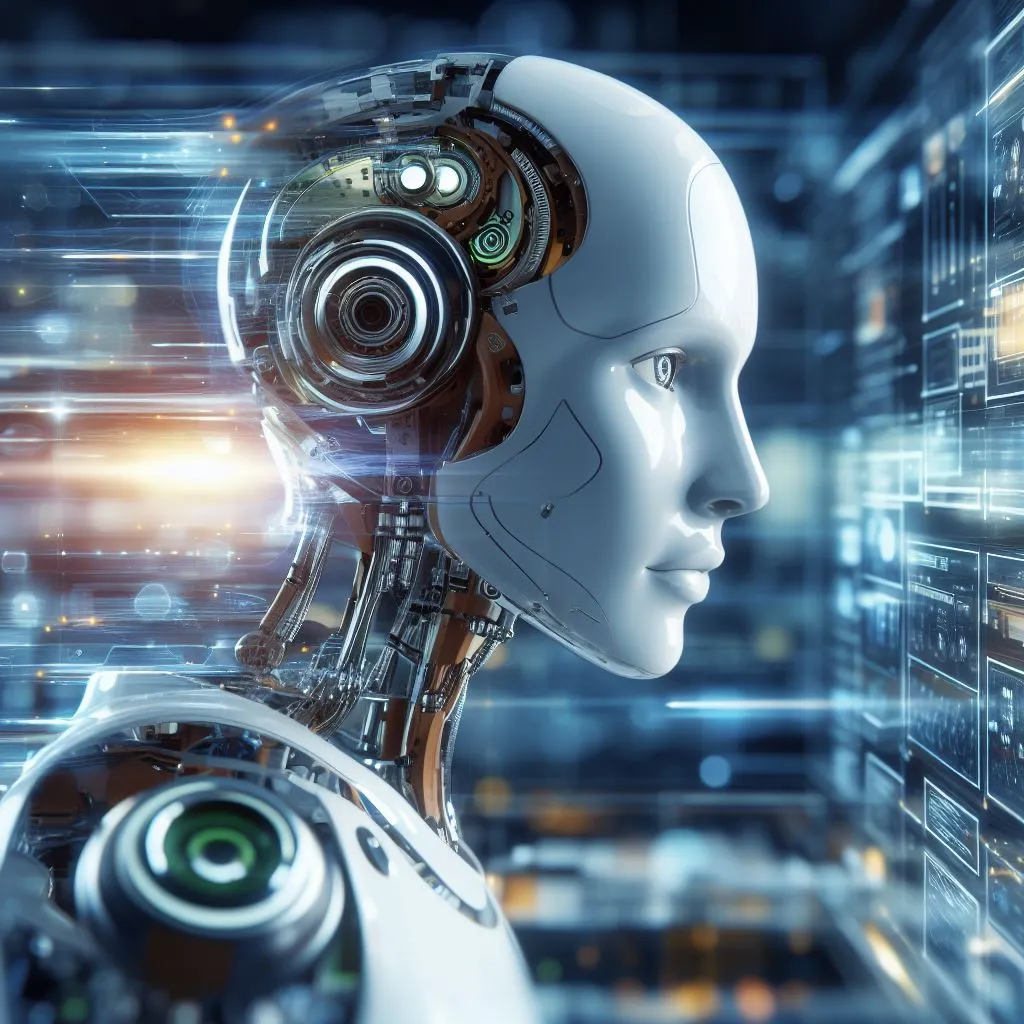
\includegraphics[height=70pt]{AI/agi.png}};
    \draw<4> (4.3, -3.3) node {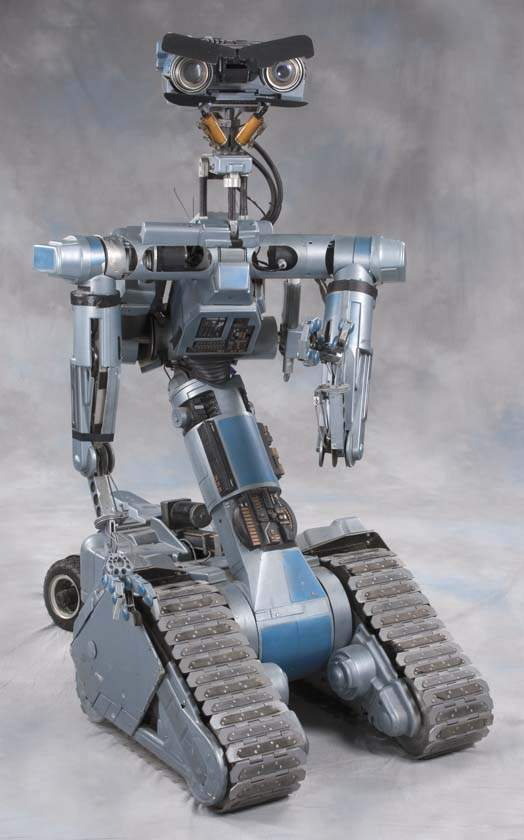
\includegraphics[height=70pt]{AI/johnny2.JPG}};
\end{tikzpicture}
\vspace{-2mm}
\begin{itemize}
    \small
    \item<1-> AI = \textit{artificial inteligence}\\ \vspace{1mm}
        -- umělá inteligence\\ \vspace{4.0mm}
    \item<2-> ML = \textit{machine learning}\\ \vspace{1mm}
        -- strojové učení\\ \vspace{4.0mm}
    \item<2-> DL = \textit{deep learning}\\ \vspace{1mm}
        -- hluboké učení\\ \vspace{4.0mm}
    \item<3-> (D)NN = \textit{(deep) neural network}\\ \vspace{1mm}
        -- (hluboká) neuronová síť\\ \vspace{4.0mm}
    \item<4-> AGI = \textit{artificial general inteligence}\\ \vspace{1mm}
        -- všeobecná umělá inteligence
\end{itemize}
\end{frame}
% AI je zkratka pro artificial inteligence, překlad umělá inteligence. Spousta lidí si pod tímto slovem představu nějaký opravdu jako inteligentní systém, často s pojený s nějakou fyzickou entitou v podobě nějakého robota. V tomto oboru se tímto pojmem však většinou označují veškeré algoritmy a programy, které mají schopnost napodobovat lidské chování a uvažování.
% Strojové učení (machine learning) je poddruh umělé inteligence. Jedná se o systémy, které mají schopnost se učit a napodobovat lidské chování, ale aniž by k tomu byly explicitně naprogramovány. Mají pouze sadu pravidel a toto chování se naučí sami na základě nějakých trénovacích dat.
% Další podtyp strojového učení je tzv. deep learning = hluboké učení, což v současnosti označuje ty nejvyspělejší metody strojového učení, které jsou schopny rozpoznávat například obličeje nebo převádět řeč na text. Označuje se jako hluboké protože se jedná zpravidla o hluboké neuronové sítě = deep neural networks,  na jejich natrénování je také zapotřebí ohromné množství trénovacích dat.
% No a pak je tu ještě další termín a to je AGI = artificial general inteligence, volný překlad všeobecná umělá inteligence. Tohoto jsme však ještě nedosáhli. Jedná se o označení pro extrémně komplexní systém, který má obrovské znalosti ve všech oborech lidského vědění, případně schopný i uvažovat či komunikovat. Často může být vázán už na nějakou konrétní fyzickou entitu, či se to dá představit třeba jako nějaký palubní počítač ve scifi filmu. Jedná se o to co se právě spoustě lidem evokuje u slovního spojení "umělá inteligence".  

\begin{frame}{\vs Strojové učení \lend}
\begin{tikzpicture}[remember picture,overlay,shift={(current page.center)}]
    \draw<1> (0, -1.6) node {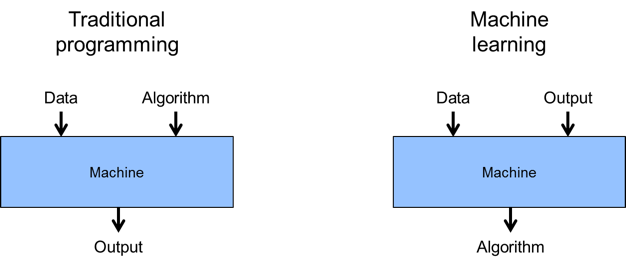
\includegraphics[width=255pt]{AI/machine-learning-1.png}};
\end{tikzpicture}
\vspace{-30mm}
\begin{itemize}
    \small
    % \item[] "Strojové učení je obor, který dává počítačům schopnost učit se, aniž by k tomu byly explicitně naprogramovány."\\ \vspace{-2.4mm}
    % \hspace{61mm}-- Arthur Samuel, 1959\\ \vspace{3.4mm}
    \item[] Strojové učení je soubor algoritmů s nastavitelnými parametry, které se pomocí trénovacích dat dokáží naučit zobecňovat a předpovídat pro dříve neviděné data.
\end{itemize}
\end{frame}
% Ještě bych řekl něco k tomu strojovému učení obecně. Citace: Arthura Samuela.
% Je tam důležitý ten aspekt, že máme nějaké trénovací data, z kterých se to chování vlastně naučíme.
% Pomocí výpočetního výkonu se optimalizují parametry toho machine learningového algoritmu, tak aby nám dal požadovaný výstup.
% To co získáme z takového procesu, který se označuje jako trénování, je právě nějaký ten natrénovaný algoritmus - třeba nějaká neuronová síť.

\begin{frame}{\vs Historický vývoj \lend}
\vspace{6mm}
\begin{itemize}
    \small
    \item[] 1952 - program hrající dámu (Arthur Samuel)\\ \vspace{0.85mm}
    \item[] 1957 - \textbf{perceptron} (Frank Rosenblatt)\\ \vspace{0.85mm}
    \item[] 1967 -  algoritmus N-nejbližších sousedů\\ \vspace{0.85mm}
    \item[] ...\\ \vspace{0.85mm}
    \item[] 1997 - Deep Blue (IBM) poráží G. Kasparova\\ \vspace{0.85mm}
    % \item[] 2006 - trénovaní neuronových sítí pomocí \textbf{zpětné propagace}\\ \vspace{0.65mm}
    \item[] 2012 - neuronová síť na rozpoznávání koček a psů (Google Brain)\\ \vspace{0.85mm}
    \item[] 2014 - systém na rozpoznávání obličejů (Facebook)\\ \vspace{0.85mm}
    \item[] 2016 - AlphaGo (Deepmind) poráží Lee Sedola\\ \vspace{0.85mm}
    \item[] 2018 - predikce struktury proteinů (AlphaFold)\\ \vspace{0.85mm}
    \item[] 2021 - velké jazykové modely (\textbf{ChatGPT})\\ \vspace{0.85mm}
    \item[] ...\\ \vspace{0.85mm}
    \item[] 2050? - všeobecná umělá inteligence (AGI)\\
\end{itemize}
\begin{tikzpicture}[remember picture,overlay,shift={(current page.center)}]
    \draw<1> (4.0, 1.6) node {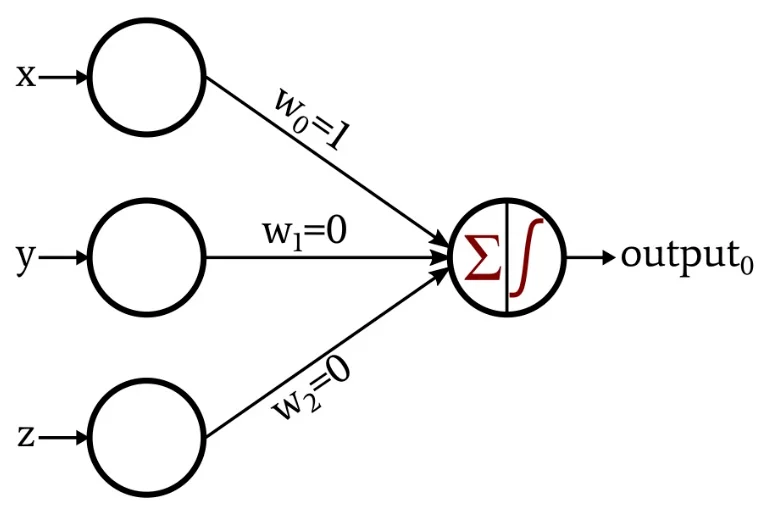
\includegraphics[width=95pt]{AI/perceptron.png}};
    \draw<1> (4.0, -2.45) node {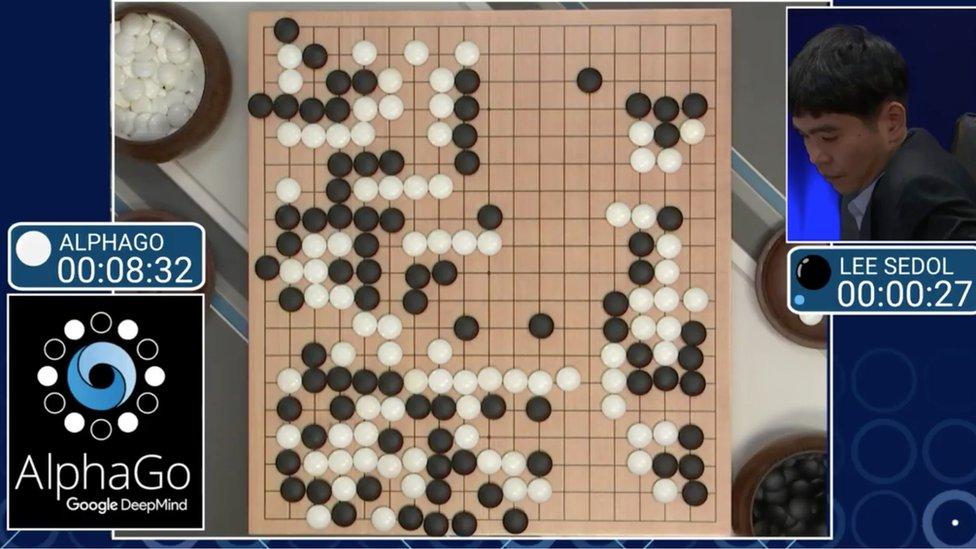
\includegraphics[width=95pt]{AI/alphago.jpg}};
\end{tikzpicture}
\end{frame}

\begin{frame}{\vs Proč až teď? - Hardware \lend}
\begin{tikzpicture}[remember picture,overlay,shift={(current page.center)}]
    \draw<1> (2.9, -0.9) node {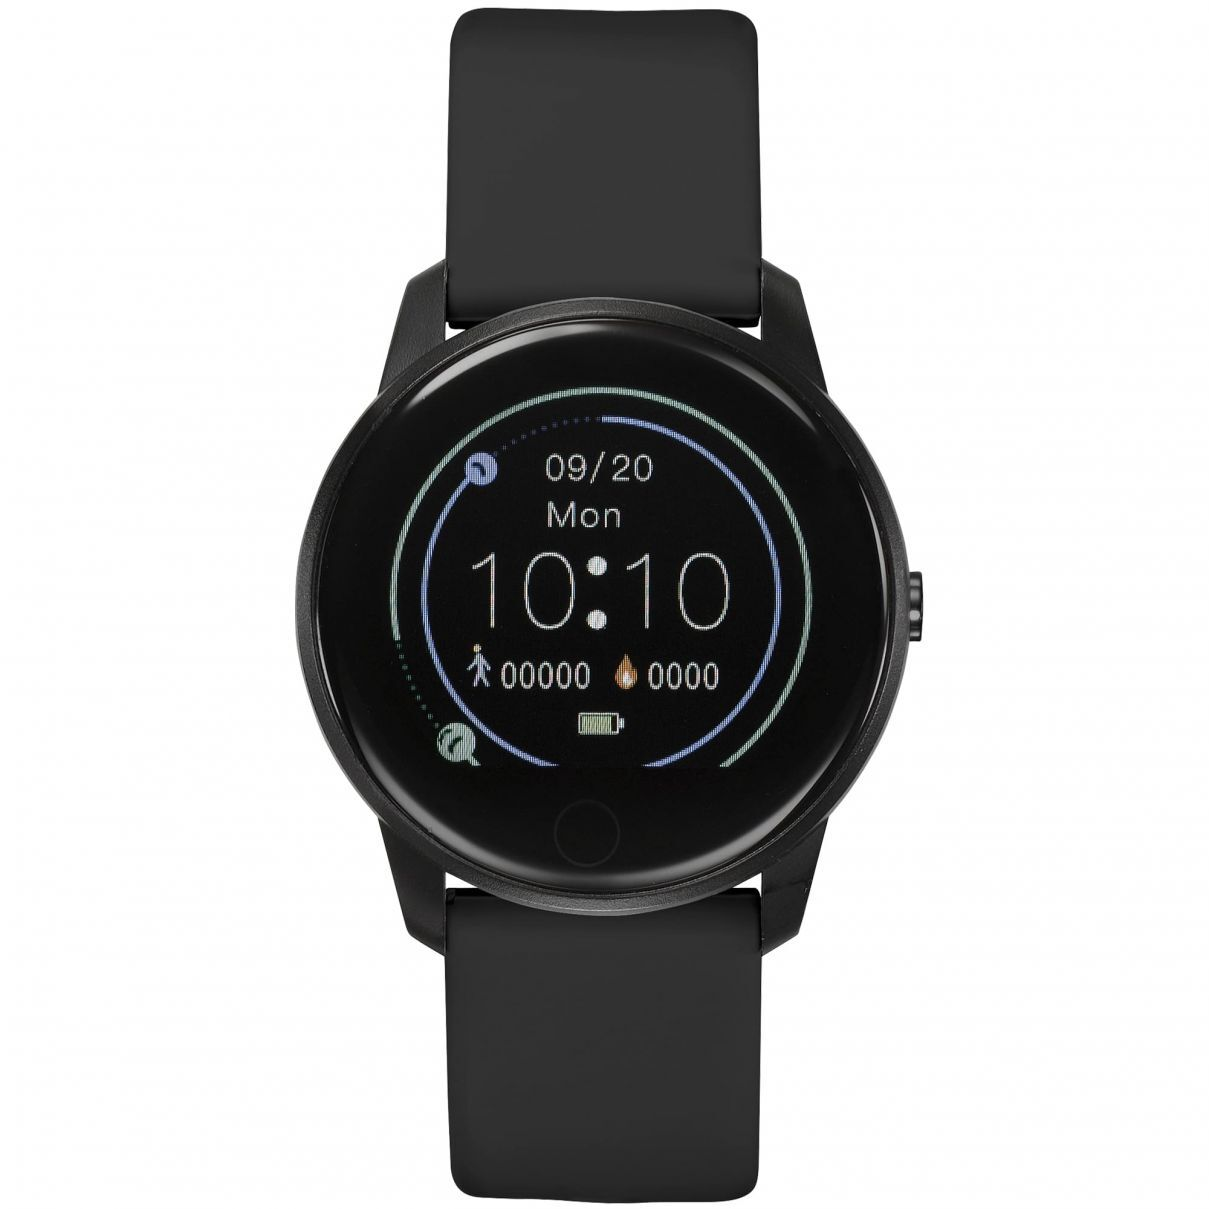
\includegraphics[width=120pt]{AI/smartwatch.jpg}};
    \draw<1> (-2.6, -0.9) node {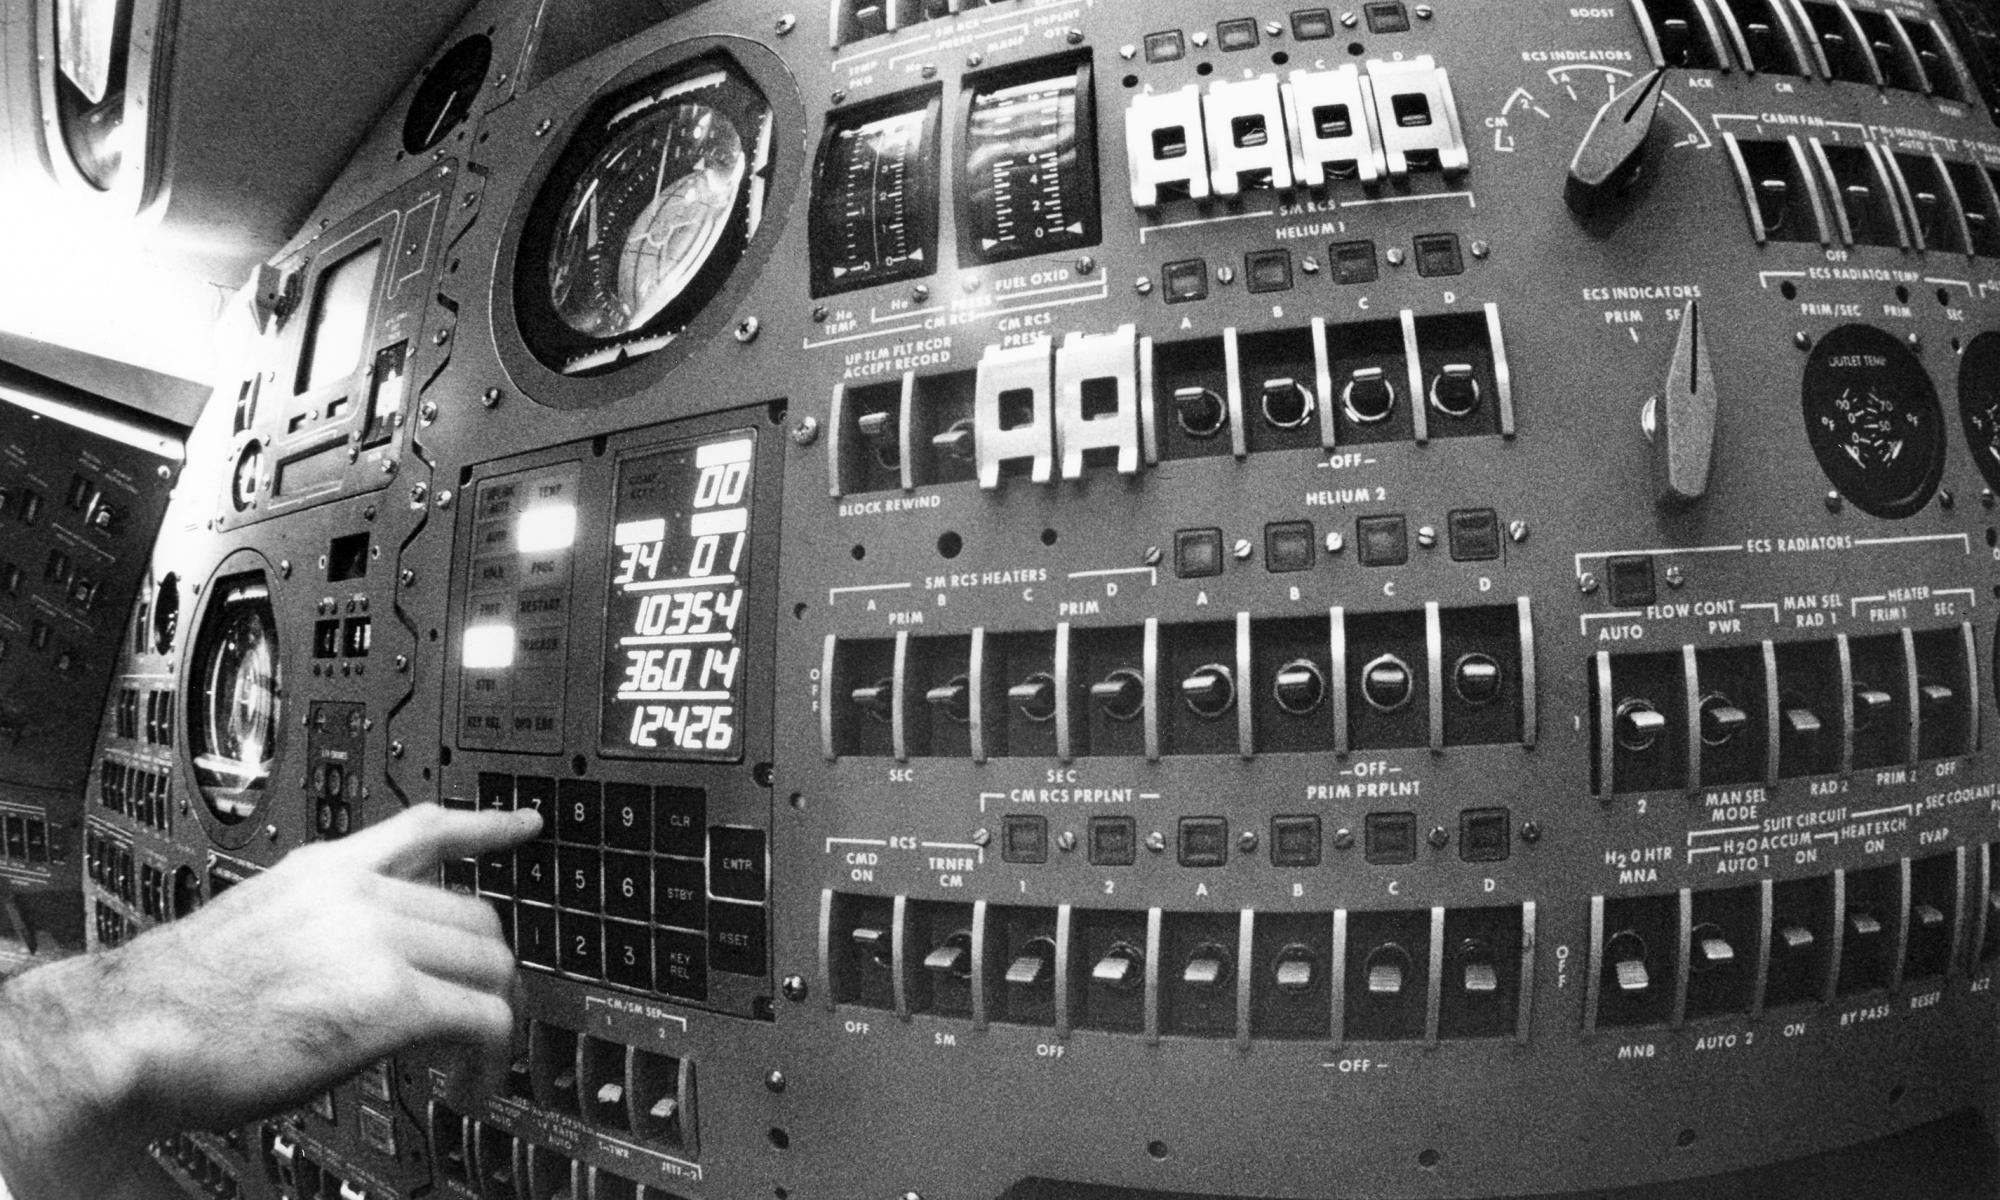
\includegraphics[width=150pt]{AI/apollo.jpg}};

    \draw<1> (-2.6, 1.5) node {\bf 1950s};
    \draw<1> (2.9, 2.0) node {\bf 2010s};

    \draw<2> (0, -1.2) node {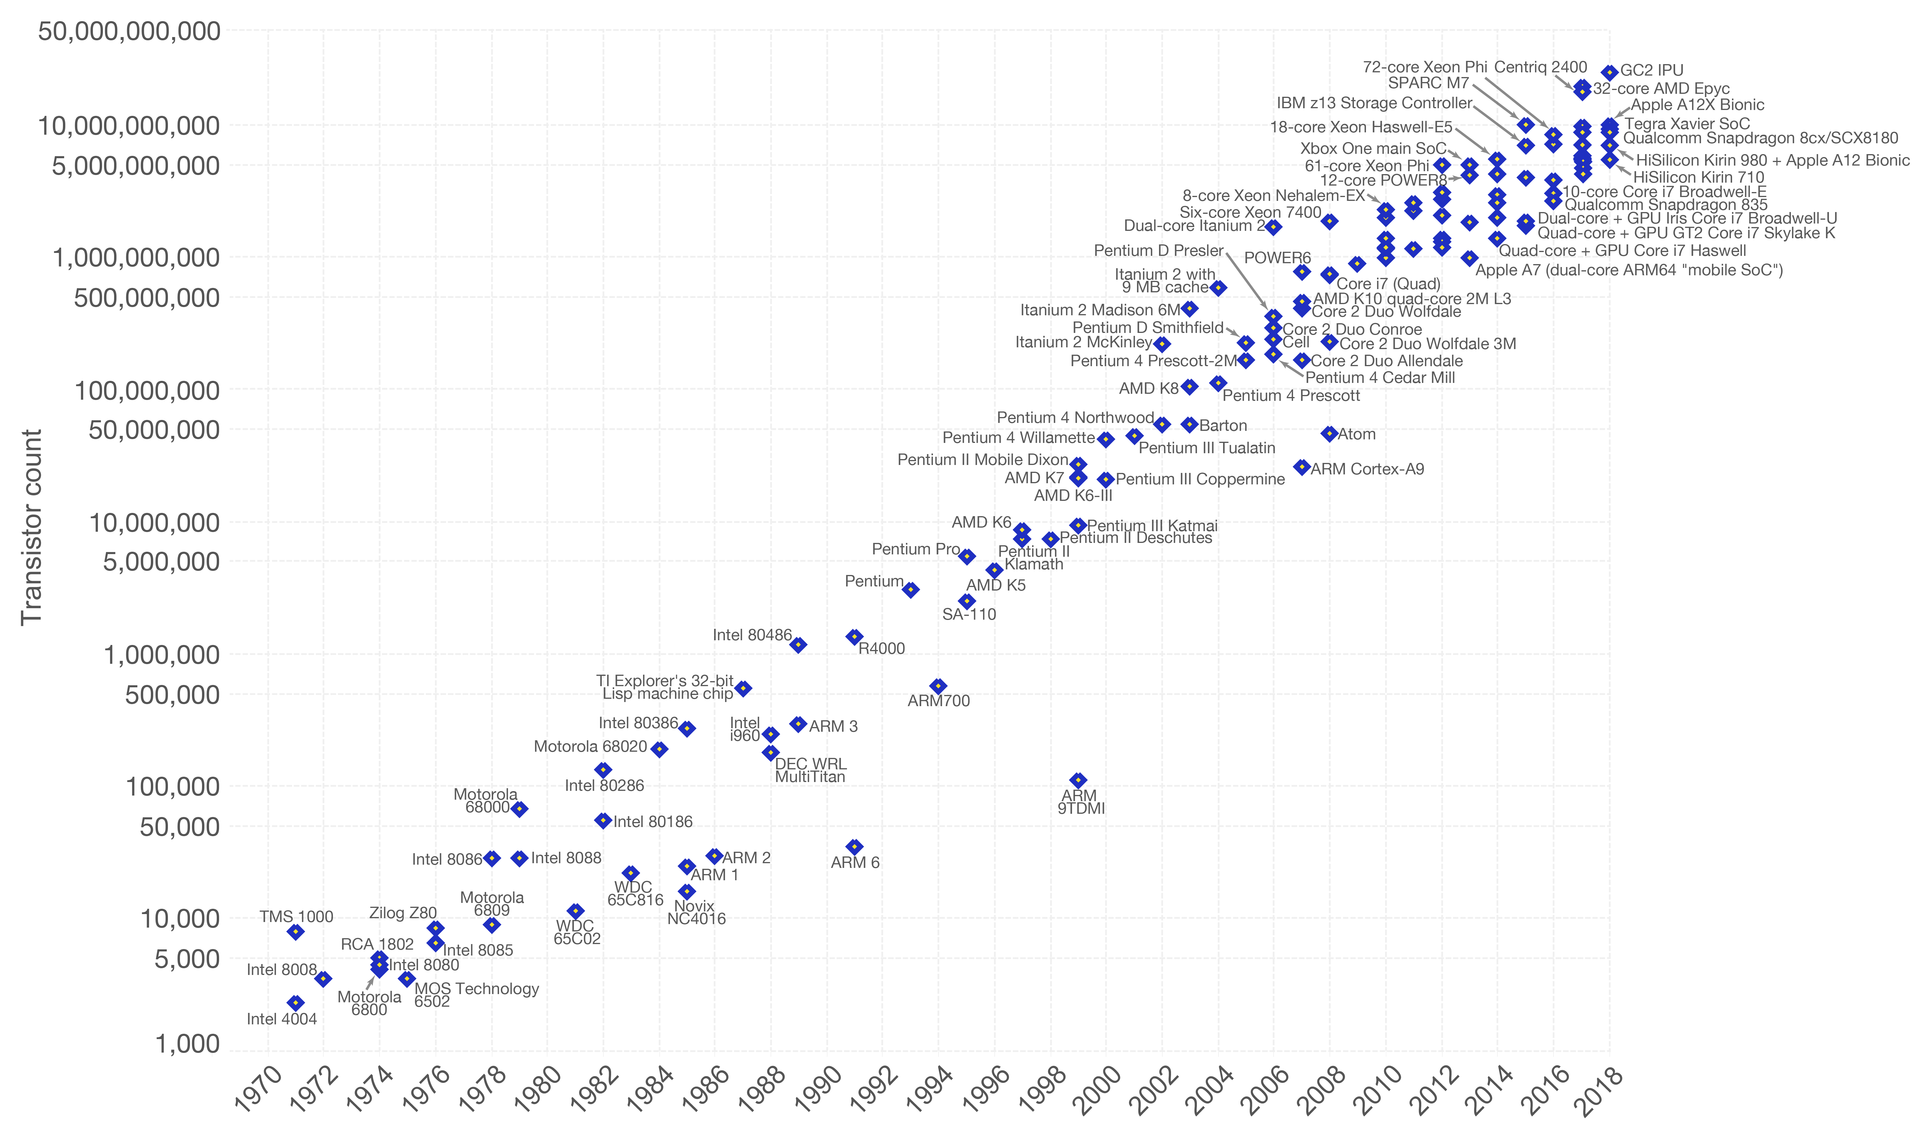
\includegraphics[width=310pt]{AI/moores_law.png}};
    \draw<2> (0, 2.5) node {Počet tranzistorů na jednom čipu - Moorův zákon};
    \draw<2> (-2, -0.5) node {$1.5\times$ za rok};

    \draw<3-> (-2.4, 2.55) node {\textbf{CPU}};
    \draw<3-> (-4.3, 1.95) node[right] {\small = central processing unit};
    \draw<3-> (-4.3, 1.35) node[right] {\small - procesor};
    \draw<3-> (-4.3, 0.75) node[right] {\small - skalární operace};
    \draw<3-> (-4.3, 0.15) node[right] {\small - rychlé výpočty (GHz)};
    \draw<4-> (2.2, 2.55) node {\textbf{GPU}};
    \draw<4-> (0.4, 1.95) node[right] {\small = graphical processing unit};
    \draw<4-> (0.4, 1.35) node[right] {\small - grafická karta};
    \draw<4-> (0.4, 0.75) node[right] {\small - vektorové operace};
    \draw<4-> (0.4, 0.15) node[right] {\small - pomaleji tisíce výpočtů};
    
    \draw<3-4> (0, -1.75) node {
\includegraphics[width=145pt]{AI/cpu_gpu_tpu_new.png}};
    \draw<3-4> (0, -3.75) node {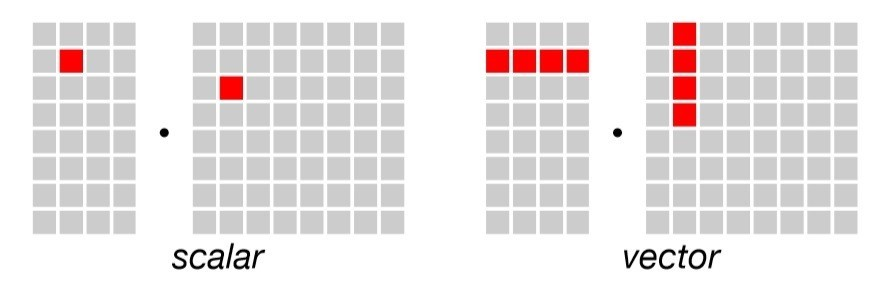
\includegraphics[width=145pt]{AI/cpu_gpu_tpu_new.jpg}};
    \draw<5-> (0, -2.4) node {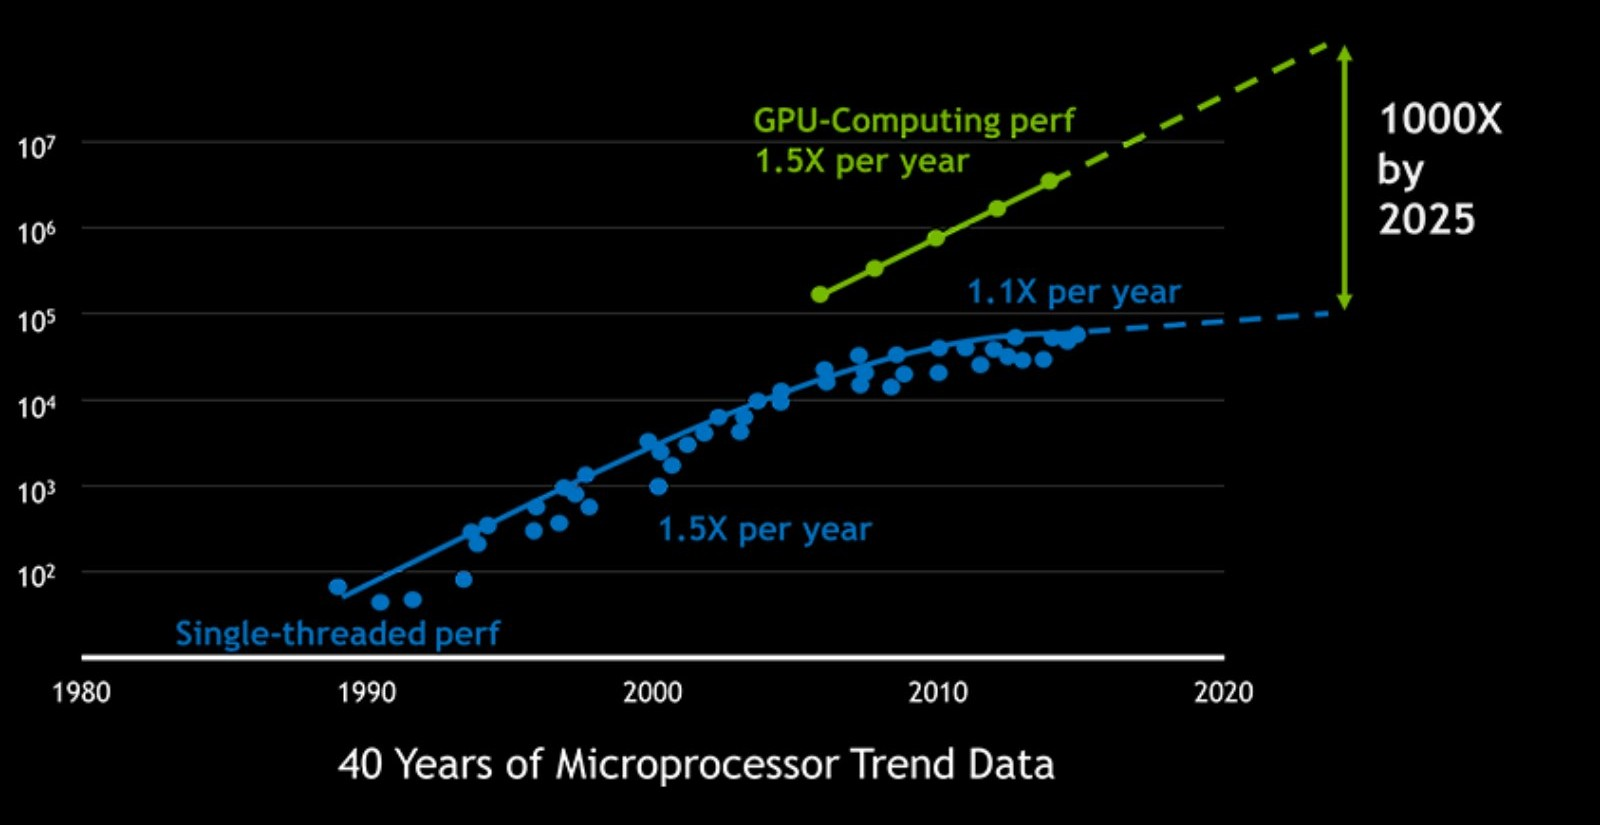
\includegraphics[width=230pt]{AI/cpu_vs_gpu.jpeg}};
\end{tikzpicture}
\end{frame}
% Je to zejména díky zdokonalení současných počítačů. Často se používá příměra, že processor v našich chytrých hodninkých je mnohem výkonější než počítač, se kterým se v 70 letech létalo na Měsíc.
% Tento vývoj se dá vyjádřit i číselně. Jak víme na základě Moorova zákona: počet tranzistorů v elektronice roste exponencielně - všimněte si, že y-ová osa má logaritmickou škálu. Znamená to tedy, že počet tranzistorů se jednou za rok znásobí 1.5x. Nicméně, v poslední době se ten nárůst už začal trošku oplošťovat.
% CPU neboli procesory však umí vykonávát pouze jednoho úkonu v daném čase. Dokáží to sice velmi rychle (5 GHz = 5 miliard úkonů za sekundu), ale pouze jeden v daném čase. V příṕadě však, že chceme například násobit dvě matice - procesor musí jít sekvenčně bod po bodu, což v případě velkých matic může být časově náročné.
% Naštěstí však existují i výpočetní jednotky jako například GPU = grafická karta (prakticky stejná jakou máme v našem stolním počítači, či notebooku). Grafická karta sestává z tísíců o něco méně výkonných mikro-procesorů - díky tomu dokáže operace jako např. násobení matic provádět vektorově, čímž se celý výpočet extrémně zrychlí. Nutno říci, že současné grafické karty jsou na takové úrovni také díky hernímu průmyslu, který vlastně financoval vývoj tohoto typu výpočetních jednotek, protože doposavad hlavní využití grafických karet bylo pro grafiku při hraní her, stříhání videa, atd.

\begin{frame}{\vs Proč až teď? - Software \lend}
\vspace{3mm}
\begin{itemize}
    \small
    \item<1-> vývoj algoritmů strojového učení\\ \vspace{2mm}
        -- stochastické hledání minima\\ \vspace{2mm}
        -- zpětná propagace\\ \vspace{2mm} 
        $\Rightarrow$ hluboké neuronové sítě\\ \vspace{5mm} 
    \item<2-> optimalizace GPU knihoven\\ \vspace{2mm}
        -- CUDA (\textbf{NVIDIA})\\ \vspace{2mm}
        -- řádové zrychlení výpočtů\\ \vspace{5mm}
    \item<3-> velmi jednoduché použití\\ \vspace{2mm}
        -- Keras (\textbf{Google}), Pytorch (\textbf{Meta})\\ \vspace{2mm}
        -- cloudové služby (Google Colab)\\
\end{itemize}
\begin{tikzpicture}[remember picture,overlay,shift={(current page.center)}]
    \draw<1-> (4.4, 1.35) node {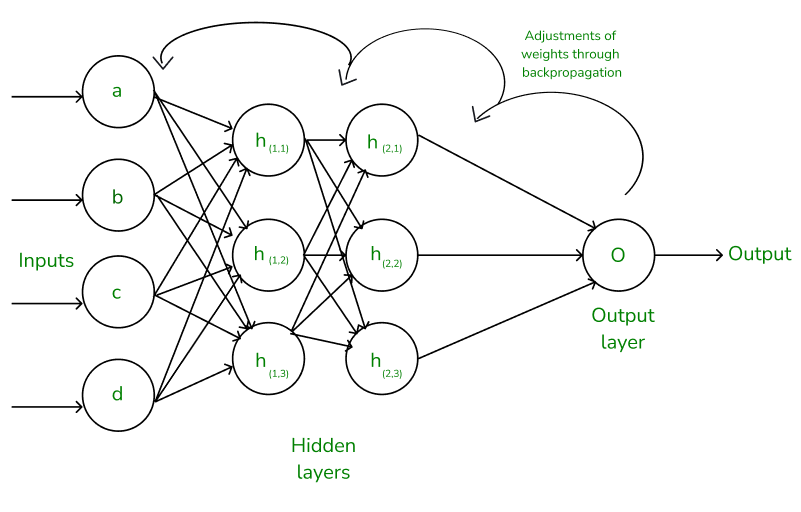
\includegraphics[width=95pt]{AI/backprop.png}};
    \draw<1-> (1.35, 1.45) node {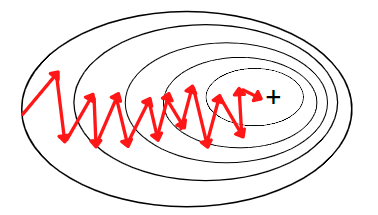
\includegraphics[width=95pt]{AI/SGD.png}};
    \draw<2-> (2.7, -0.85) node {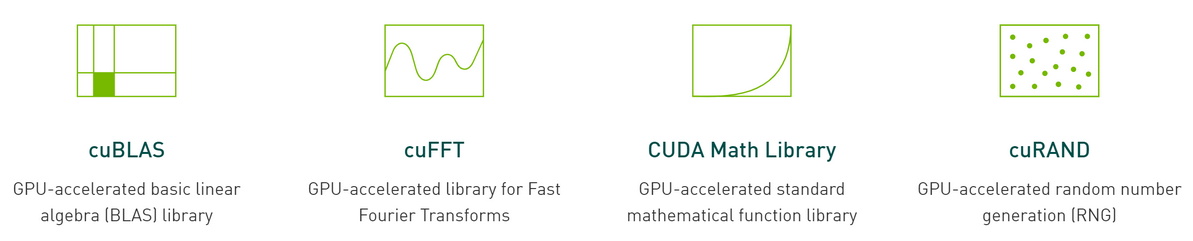
\includegraphics[width=195pt]{AI/cuda.png}};
    \draw<3-> (2.7, -3.20) node {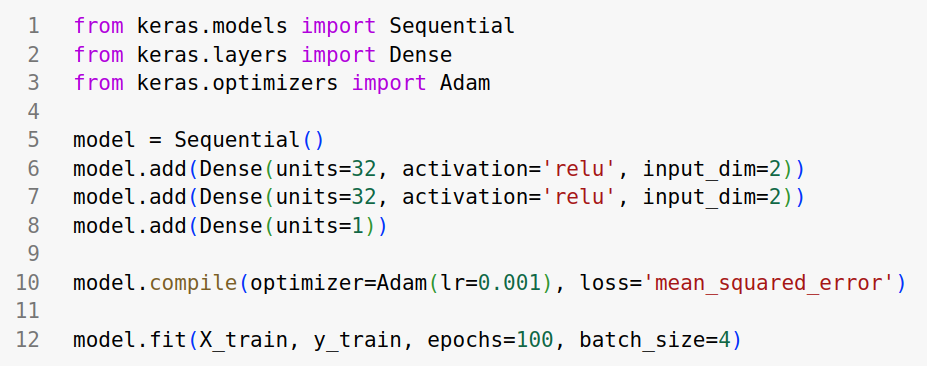
\includegraphics[width=140pt]{AI/keras.png}};
\end{tikzpicture}
\end{frame}
% Text

\begin{frame}{\vs Proč až teď? - Data \lend}
\vspace{2mm}
\begin{itemize}
    \small
    \item<1,3-> záznamová zařízení\\ \vspace{2.5mm}
        -- fotoaparáty, mobilní telefony\\ \vspace{2.5mm}
        -- bezpečnostní/palubní kamery\\ \vspace{4mm}
    \item<1,3-> chytrá zařízení\\ \vspace{2.5mm}
        -- IoT = \textit{internet of things}\\ \vspace{2.5mm}
        -- hodinky, pračky, domácnost..\\ \vspace{4mm}
    \item<3-> internet \& digitalizace\\ \vspace{2.5mm}
        -- veřejné databáze (Common Crawl)\\ \vspace{2.5mm}
        -- sociální sítě (Facebook, Instagram)\\ \vspace{2.5mm}
        -- cloudové služby (Google, GitHub)\\ \vspace{2.5mm}
        % -- (ne)publikovaný software (GitHub)\\
\end{itemize}
\begin{tikzpicture}[remember picture,overlay,shift={(current page.center)}]
    \draw<1,3-> (2.85, 0.9) node {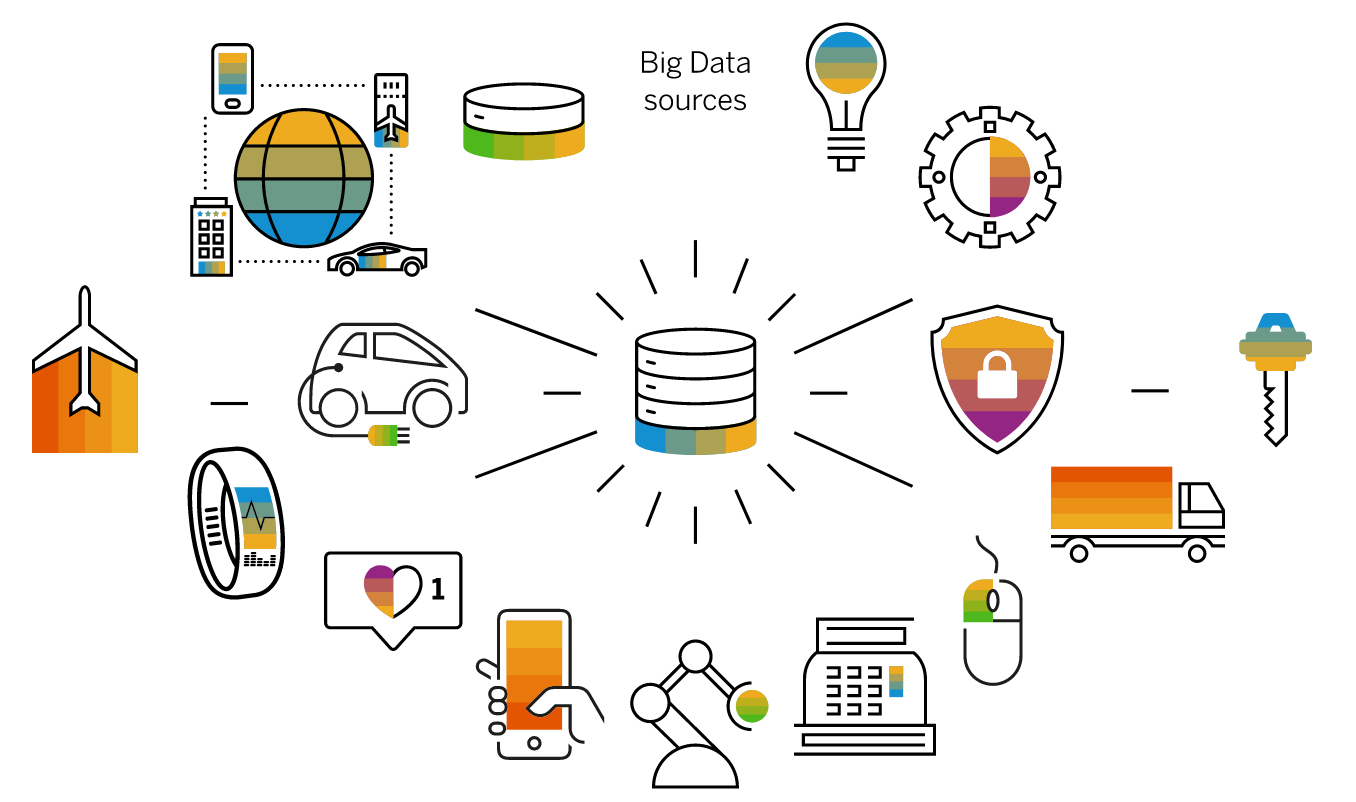
\includegraphics[width=170pt]{AI/big_data.png}};
    \draw<2> (0, -0.6) node {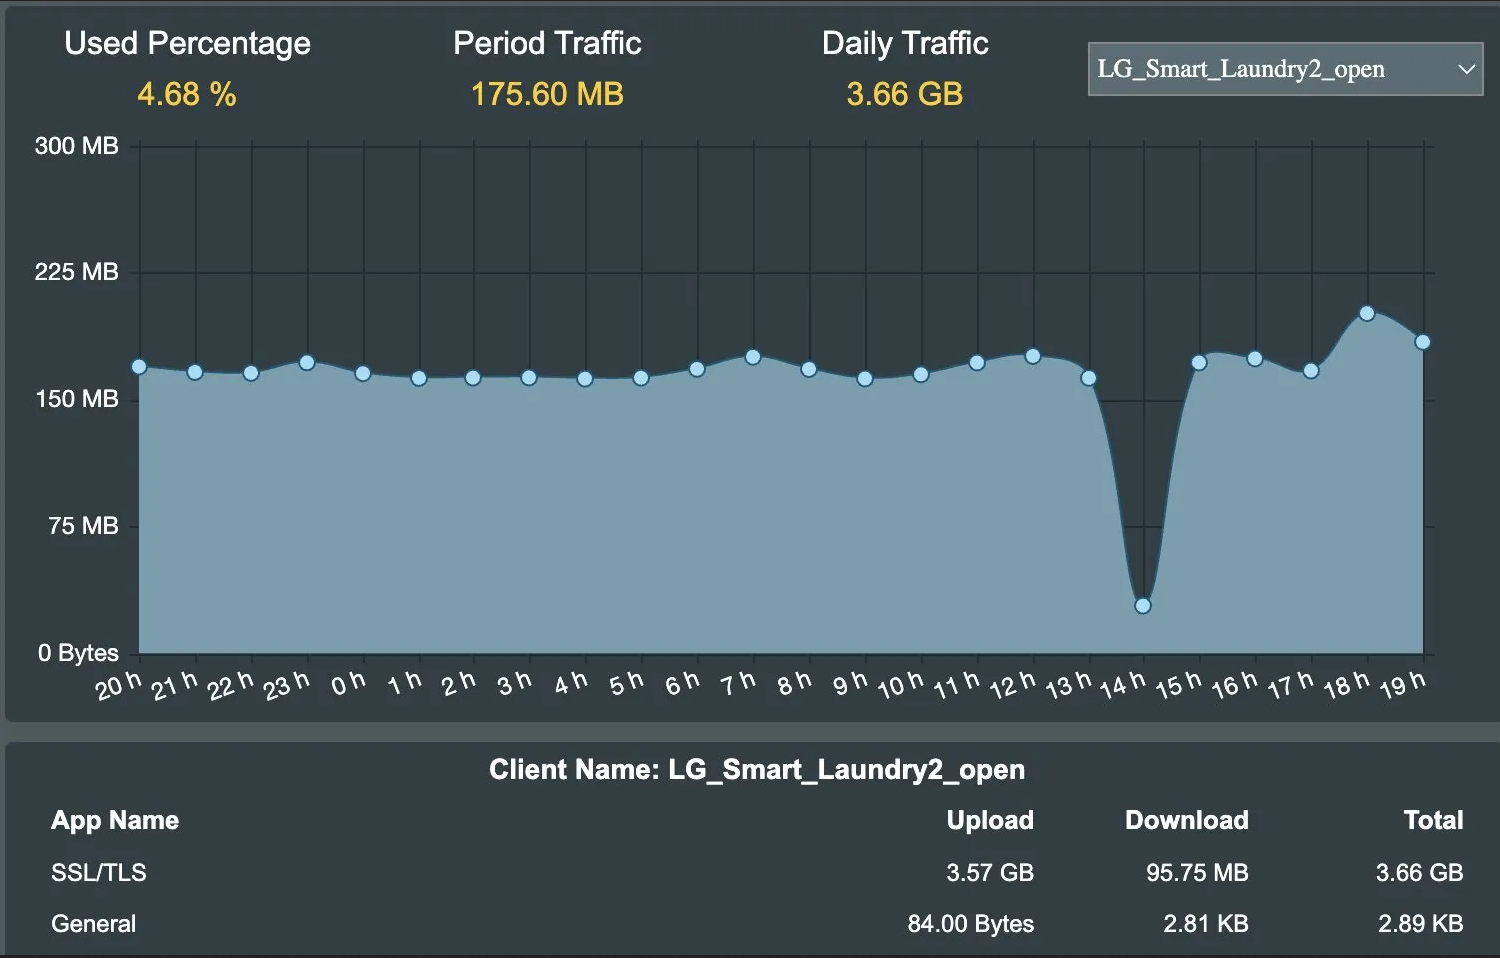
\includegraphics[width=315pt]{AI/pracka.png}};
    \draw<2>[color=red,line width=1pt] (1.77, -3.32) ellipse (0.43cm and 0.43cm);
    \draw<3-> (3.0, -2.65) node {
\includegraphics[width=120pt]{AI/social_network.jpg}};
\end{tikzpicture}
\end{frame}
% Ale záznamová zařízení sami o sobě nám nestačí - potřebujeme je ještě nějak sdílet a k tomu nám pomohl internet a obecně digitalizace.
% Dobře víme, že tyhle obří firmy se s ochranou dat uživatelů zase tak moc nepářou.


\section{Neuronová síť}

\begin{frame}{\vs Neuron\lend}
\vspace{0mm}
\begin{itemize}
    \item<1-> umělý neuron = základní stavební jednotka\\ \vspace{2mm}
        -- každý neuron má vstup $x_i$\\ \vspace{2mm}
        -- každé spojení má váhu $w_i$\\ \vspace{2mm}
        -- každý neuron má tzv. bias $b$\\ \vspace{2mm}
    \item<2->[]-- aktivační funkce $f$ (sigmoid, ReLU)\\ \vspace{3mm}
    \item<4-> neurony se spojují do vrstev\\ \vspace{2mm}
        -- vstupní (data) a výstupní vrstva (klasifikace/regrese)\\ \vspace{2mm}
    \item[]<5> -- skryté vrstvy\\ \vspace{2mm}
        \hspace{4mm} -- husté vrstvy\\ \vspace{2mm}
        \hspace{4mm} -- konvoluční\\ \vspace{2mm}
        \hspace{4mm} -- reziduální\\ \vspace{2mm}
\end{itemize}
\begin{tikzpicture}[remember picture,overlay,shift={(current page.center)}]
    \draw<1-3> (0, -2.55) node {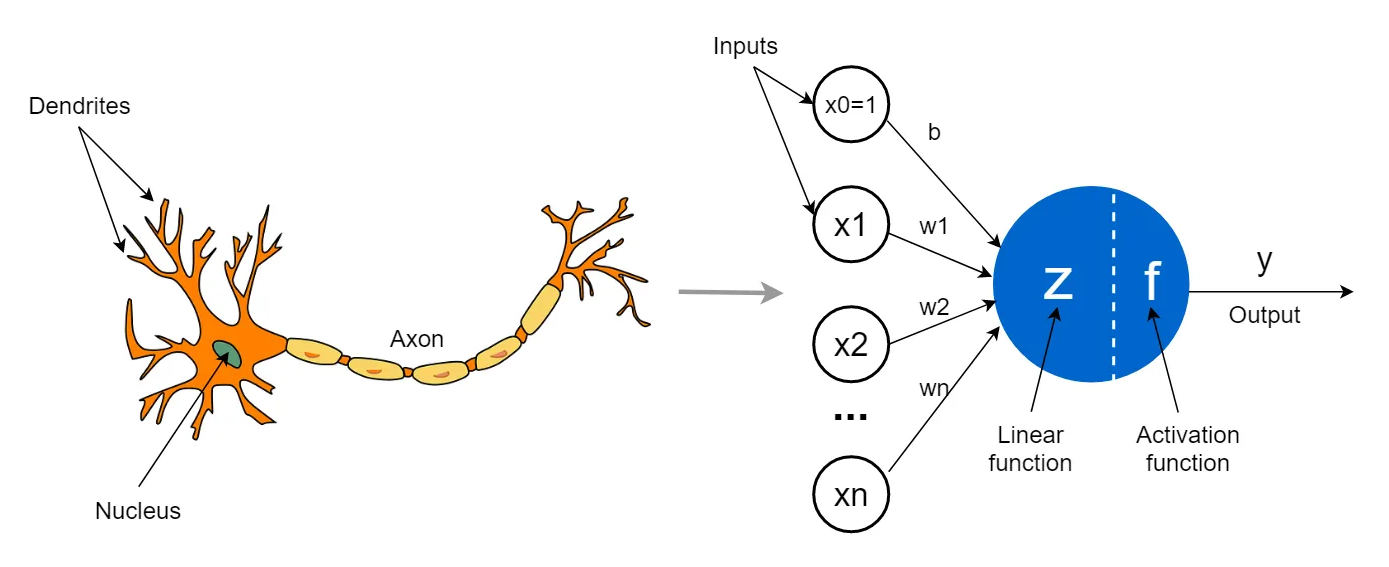
\includegraphics[width=280pt]{AI/neuron.png}};
    \draw<2-> (3.5, 1.7) node {$y = f \left( \sum_i w_i x_i + b \right)$};
    \draw<2-> (3.95, 2.1) node[rotate=270] {\Large $\Biggr\{$};
    \draw<2-> (3.95, 2.4) node {$z$};
    \draw<3-> (3.6, 0.15) node {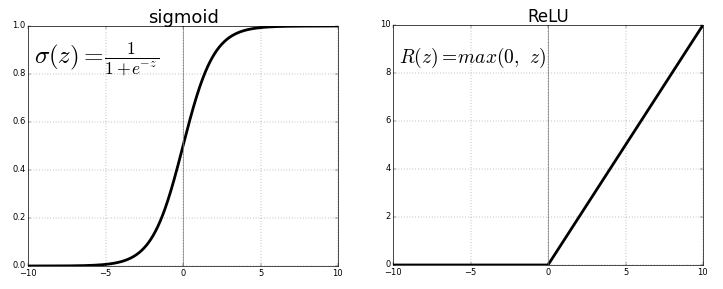
\includegraphics[width=130pt]{AI/sigmoid_relu.png}};
    \draw<4-> (2.5, -0.95) node {\tiny klasifikace};
    \draw<4-> (4.7, -1.03) node {\tiny regrese};

    \draw<5-> (-0.8, -3.35) node {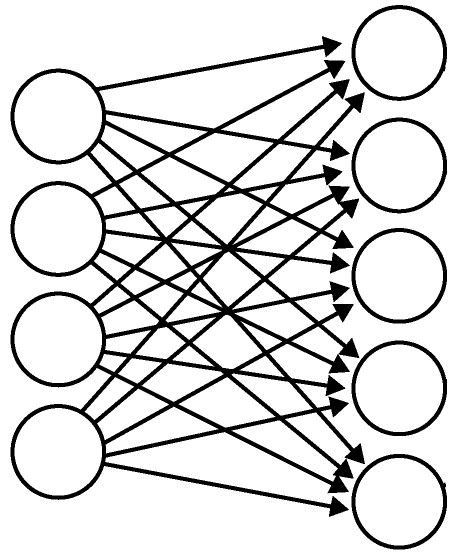
\includegraphics[height=70pt]{AI/husta_vrstva.png}};
    \draw<5-> (4.7, -3.2) node {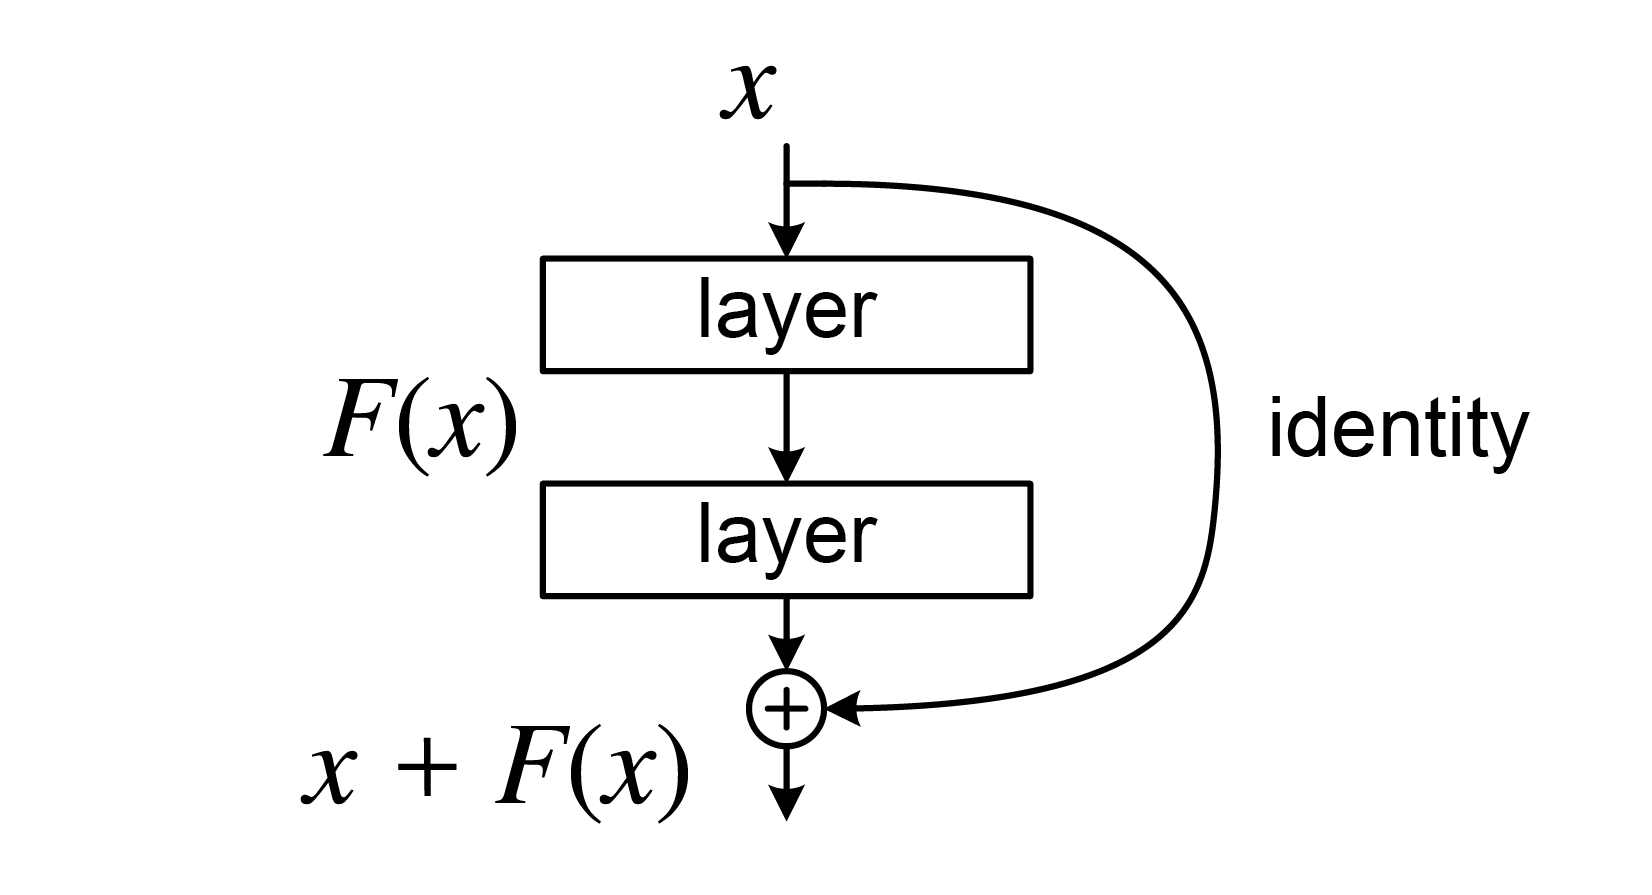
\includegraphics[height=55pt]{AI/residual.png}};
    \draw<5-> (2.1, -3.2) node {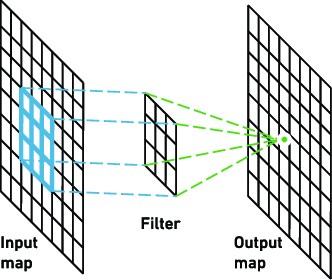
\includegraphics[height=55pt]{AI/convolutional-layer.png}};
\end{tikzpicture}
\end{frame}
% Vstupní vrstva zpravidla nemá aktivační funkci - ta reprezentuje vlastně ty naše data, které tam vkládáme.
% Výstupní vrstva má aktivační funkci nastavenou podle účelu neuronové sítě. Pokud chceme dělat například binární klasifikaci (pes vs kočka, proměnná vs nepromenná hvězda), či tzv. regresi. V takovém případě je výstupem číslo - například reprezentující nějakou fyzikální veličinu (například teplota té hvězdy).

% V případě binární klasifikace se více hodí aktivační funkce sigmoid, která nabývá hodnot od nuly (kočka) do jedničky (pes). Samozřejmě počítač neví co je to kočka nebo pes, takže je potřeba jednotlivé třídy nějak reprezentovat.

% V případě regrese se více hodí aktivační funkce ReLU, případně pouze lineární závislost, pokud veličina může nabývat i záporných hodnot (což není případ teploty). 

\begin{frame}{\vs Neuronová síť \lend}
\vspace{57mm}
\begin{itemize}
\large
\item[]<3> \hspace{23mm} \begin{pmatrix}
w_{11} & \cdots & w_{1\text{n}}\\
\vdots & \ddots & \vdots\\
w_{\text{m}1} & \cdots & w_{\text{mn}}
\end{pmatrix}
\vspace{-17mm}
\item[]<3> \hspace{78mm} \begin{pmatrix}
b_{1}\\
\vdots\\
b_{m}
\end{pmatrix}
% \vspace{-17mm}
% \item[]<2> \hspace{88mm} \begin{pmatrix}
% w_{1}\\
% \vdots\\
% w_{m}
% \end{pmatrix}
\end{itemize}
\begin{tikzpicture}[remember picture,overlay,shift={(current page.center)}]
\large
    \draw<1-> (0.1,0.5) node {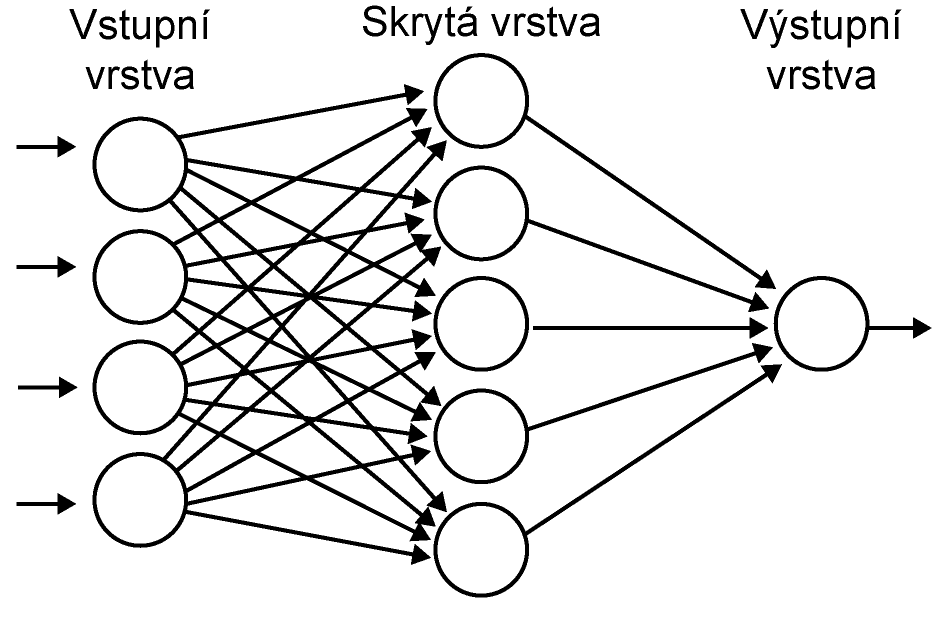
\includegraphics[width=190pt]{AI/neuronova_sit.png}};
    \draw<1-5> (-3.65,1.65) node {\large $x_1$};
    \draw<1-5> (-3.65,0.82) node {\large $x_2$};
    \draw<1-5> (-3.65,-0.09) node[rotate=90] {\large $...$};
    \draw<1-5> (-3.65,-0.92) node {\large $x_{\text{n}}$};
    \draw<1-5> (-3.65,-2.0) node {\large $\vec{X}_{\text{n}}$};
    \draw<2-6> (-1.35,-1.70) node {\large $\textbf{w}_1,\vec{b}_1$};
    \draw<3> (-3.47,-3.55) node {\large $\textbf{w}_1=$};
    \draw<3> (2.05,-3.55) node {\large $\vec{b}_1=$};
    \draw<1-6> (0.2,-2.07) node {\large $\vec{h}_{\text{m}}$};
    \draw<2-6> (1.60,-1.70) node {\large $\textbf{w}_2,\vec{b}_2$};
    \draw<1-5> (3.70,0.38) node {\large $y$};

    \draw<4-> (-2.1,-3.55) node {$\vec{h} = f_1 \left( \textbf{w}_1 \vec{X} + \vec{b}_1\right)$};
    \draw<5-> (2.1,-3.55) node {$y = f_2 \left( \textbf{w}_2 \vec{h} + \vec{b}_2 \right)$};

    \draw<6-> (-4.7,0.4) node {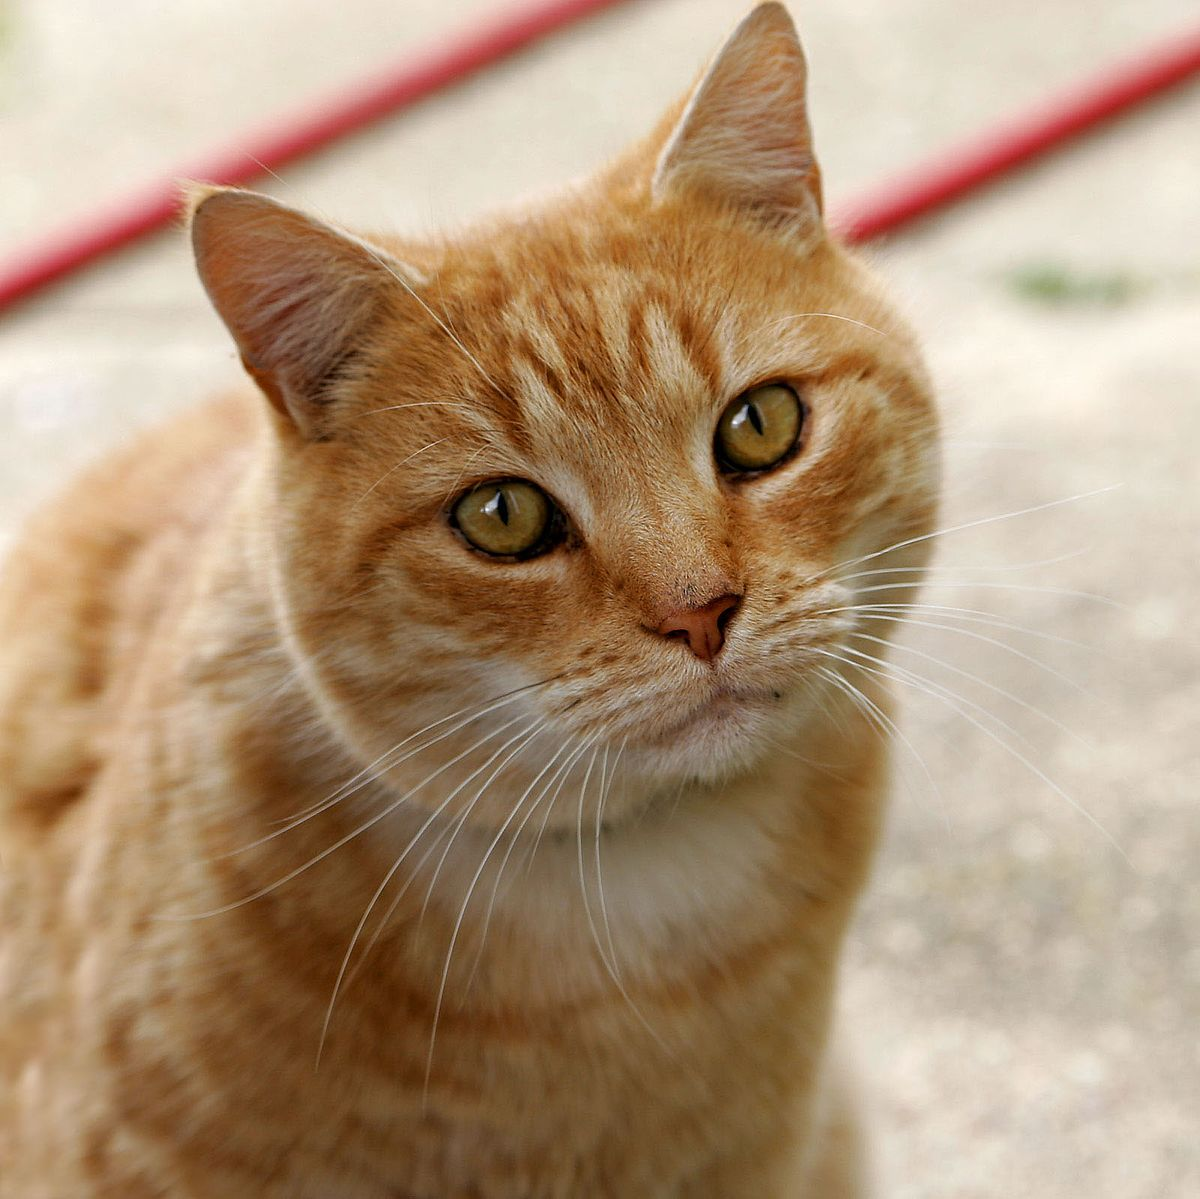
\includegraphics[width=72pt]{AI/cat.jpg}};

    \draw<6> (3.7,1.2) node[right] {\scriptsize (po trénování)};
    \draw<6> (3.9,0.6) node[right] {\scriptsize 93\% kočka};
    \draw<6> (3.9,0.1) node[right] {\scriptsize 7\% pes};

    \draw<7> (2.6,-2.1) node {\scriptsize náhodné};
    \draw<7> [->,line width=0.25mm] (2.6,-2.35) -- (3.1, -3.0);
    \draw<7> [->,line width=0.25mm] (2.6,-2.35) -- (2.2, -3.0);
    \draw<7> (-1.7,-2.1) node {\scriptsize náhodné};
    \draw<7> [->,line width=0.25mm] (-1.7,-2.35) -- (-1.2, -3.0);
    \draw<7> [->,line width=0.25mm] (-1.7,-2.35) -- (-2.1, -3.0);
    \draw<7> (4.25,-1.25) node[rotate=48] {
\includegraphics[width=43pt]{AI/arrow.png}};
    \draw<7> (3.25,1.2) node[right] {\scriptsize (před trénováním)};
    \draw<7> (3.7,0.6) node[right] {\scriptsize 48\% kočka};
    \draw<7> (3.7,0.1) node[right] {\scriptsize 52\% pes};
\end{tikzpicture}
\end{frame}
% Jednotlivá čísla a neurony nemají zase takovou důležitost a shopnost, ale jako celek to tvoří poměrně komplexní systém, který je schopný zdánlivě až imitovat určité aspekty lidského chování. Jak něco takového vůbec může fungovat? Systém je velmi komplexní - má ?? trénovatelných parametrů a navíc je silně nelineární.
% Neuronová síť je velmi komplexní a nelineární matematická operace.

\begin{frame}{\vs Trénování \lend}
\vspace{1mm}
\begin{itemize}
    \small
    \item<1-4> \textit{supervised learning} = "učení s učitelem"\\ \vspace{1.8mm}
        -- pro každé $\vec{X}$ máme odpovídající $y$\\ \vspace{1.8mm}
        -- velké množství snímků ($\gtrsim 10^4$)\\ \vspace{3.5mm}
    \item<3-4> cílem je najít zobrazení $F(\vec{X}) = y$\\ \vspace{3.5mm}
    \item<4-4> \textit{loss function} - funkce penalizující špatné predikce \\ \vspace{1.8mm}
        -- regrese - root mean square error (RMSE)\\ \vspace{1.8mm}
        -- klasifikace - binary crossentropy\\ \vspace{3.5mm}
    \item<4-4> stochastické hledání minima (SGD)\\ \vspace{1.8mm}
        -- postupujeme po krocích (batchích)\\ \vspace{3.5mm}
    \item<4-4> \textit{backpropagation} = zpětná propagace\\ \vspace{1.8mm}
        -- aktualizujeme váhy $\textbf{w}$ a biasy $\vec{b}$\\ \vspace{4mm}
\end{itemize}
\begin{tikzpicture}[remember picture,overlay,shift={(current page.center)}]
    \draw<2-4> (4.5,2.35) node {\scriptsize kočka (1)};
    \draw<2-4> (4.5,1.2) node {\includegraphics[width=50pt]{AI/cat.jpg}};
    \draw<2-4> (2.4,2.35) node {\scriptsize pes (0)};
    \draw<2-4> (2.4,1.2) node {\includegraphics[width=50pt]{AI/dog.jpg}};

    \draw<4> (3.35, -2.65) node {\includegraphics[width=115pt]{AI/SGD.png}};
    % \draw<4> (3.35, -2.65) node {\tiny $$\mathcal{L}(y, \hat{y}) = -\frac{1}{N} \sum_{i=1}^{N} \left[ y_i \log(\hat{y}_i) + (1 - y_i) \log(1 - \hat{y}_i) \right]$$};

    \draw<8-> (-4.1,-3.15) node {\includegraphics[width=110pt]{CADET/loss_curve.png}};

    % \draw<1> (2.0, 1.5) node {$F(x) = y$};
    \draw<5-> (0.1,-0.2) node {\includegraphics[width=190pt]{AI/neuronova_sit.png}};
    \draw<5-> (-4.2,-0.2) node {$\vec{X}_{\text{trénink}}$};
    \draw<5-> (4.3,-0.3) node {$\vec{y}_{\text{predikce}}$};
    \draw<6-> [->,line width=0.25mm] (4.1,-0.75) -- (3.9, -1.5);
    \draw<6-> (4.1,-2.0) node {loss\,($\vec{y}_{\text{predikce}}$, $\vec{y}_{\text{trénink}}$)};
    \draw<7-> [->,line width=0.25mm] (3.6,-2.55) -- (2.6, -3.2);
    \draw<7-> (-1.15,-3.23) node {\Large $\textbf{w}_1,\,\vec{b}_1$};
    \draw<7-> [->,line width=0.25mm] (0.5,-3.3) -- (-0.2, -3.3);
    \draw<7-> (1.45,-3.23) node {\Large $\textbf{w}_2,\,\vec{b}_2$};
\end{tikzpicture}
\end{frame}
% Samozřejmě nefunguje to samo od sebe. Takovou neuronovou síť je nejdříve potřeba natrénovat, protože ty hodnoty w a b jsou na začátku inicializovány úplně náhodně. Takže kdybychom chtěli používat nenatrénovanou neurovou síť, tak budeme dostávat prakticky náhodné predikce. Například jako kdybychom si hodili mincí, jestli to na obrázku je kočka nebo pes.

\begin{frame}{\vs Použití \lend}
\vspace{-25mm}
\begin{itemize}
    \small
    \item<1-> omezené použití - klasifikátor psů a koček zná jen kočky a psy\\ \vspace{3mm}
    \item<1-> jen určitý typ vstupu (snímek $128\times128\times3$) a výstupu ($0-1$)\\ \vspace{3mm}
    \item<3-> pro použití na slony je potřeba přidat výstupní neurony a přetrénovat
\end{itemize}
\begin{tikzpicture}[remember picture,overlay,shift={(current page.center)}]
    \draw<1-> (0.2,-2.3) node {\includegraphics[width=190pt]{AI/neuronova_sit.png}};

    \draw<1> (-4.7,-2.4) node {\includegraphics[width=72pt]{AI/cat.jpg}};
    \draw<1> (3.7,-2.2) node[right] {\scriptsize 93\% kočka};
    \draw<1> (3.7,-2.7) node[right] {\scriptsize 7\% pes};

    \draw<2-> (-4.7,-2.4) node {\includegraphics[width=72pt]{AI/elephant.jpg}};
    \draw<2> (3.7,-2.2) node[right] {\scriptsize 56\% kočka};
    \draw<2> (3.7,-2.7) node[right] {\scriptsize 44\% pes};

    \draw<3-> (2.87,-1.6) node {\includegraphics[width=34pt]{AI/output_neuron.png}};
    \draw<3-> (2.87,-3.2) node {\includegraphics[width=34pt]{AI/output_neuron.png}};
    \draw<3> (3.7,-1.6) node[right] {\scriptsize 3\% kočka};
    \draw<3> (3.7,-2.43) node[right] {\scriptsize 7\% pes};
    \draw<3> (3.7,-3.2) node[right] {\scriptsize 90\% slon};
\end{tikzpicture}
\end{frame}
% Je potřeba si však uvědomit, že ten systém je extrémně omezený a použitelný pouze na to na co byl natrénován a to jsou fotky psů a koček. Pokud bysme klasifikátoru koček a psů dali fotku slona, tak by nám opět vyhodil pouze číslo mezi 0 a 1 (ale pro nás je 0 kočka a 1 pes). Pokud bysme chtěli klasifikovat i slony, museli bychom neurovou síť se třemi výstupy - jeden pro každou třídu, a tu bysme museli natrénovat pomocí fotek koček, psů, ale i slonů.


\section{Využití AI}

\begin{frame}{\vs Co je a co není AI? \lend}
\begin{tikzpicture}[remember picture,overlay,shift={(current page.center)}]
    % % \draw<2-4> (3.0, -3.0) node {\includegraphics[height=80pt]{AI/ML_vs_DL.jpg}};
    % \draw<2> (2.1, -3.3) node {\includegraphics[height=70pt]{AI/agi.png}};
    \draw<1-> (0, 2.55) node {\textbf{spam filtr}};
    \draw<1-> (-2.8, 1.95) node {\small klíčová slova};
    \draw<1-> (-2.8, 1.2) node {\small \uv{výhra}};
    \draw<1-> (-2.8, 0.75) node {\small \uv{zdarma}};
    \draw<1-> (-2.8, 0.25) node {\small \uv{Nigerijský princ}};
    \draw<1-> (3.2, 0.85) node {\includegraphics[height=80pt]{AI/spam_filter.png}};
    \draw<1-> (2.7, 1.95) node {\small detekce anomálií};

    \draw<2-> (0, -0.65) node {\textbf{automatické otevírání dveří}};
    \draw<2-> (-2.8, -1.25) node {\small fotobuňka};
    \draw<2-> (2.8, -1.25) node {\small rozpoznání obličejů};
    \draw<2-> (-2.8, -3.05) node {\includegraphics[height=80pt]{AI/automatic_door.jpg}};
    \draw<2-> (2.8, -3.05) node {\includegraphics[height=80pt]{AI/facial_recognition.png}};
\end{tikzpicture}
\vspace{-1mm}
% \begin{itemize}
%     \item filtr spamu\\
%     \item vyhledávání klíčových slov, 
%     \item automatické otevírání dveří, fotobuňka\\
%     \item rozpoznávání obličejů
% \end{itemize}
\end{frame}


\begin{frame}{\vs Analýza zvuku \& obrazu \lend}
\vspace{1mm}
\begin{itemize}
    \item<1-> rozpoznání řeči\\ \vspace{2mm}
        -- domácí asistenti\\ \vspace{2mm}
        -- hlasové ovládání\\ \vspace{2mm}
        -- převod řeči na text\\ \vspace{5.5mm}
    \item<2-> rozpoznávání objektů, obličejů\\ \vspace{2mm}
        -- zdravotnictví\\ \vspace{2mm}
        -- bezpečnostní systémy\\ \vspace{4.5mm}
    \item<3-> obrazová segmentace\\ \vspace{2mm}
        -- automatizace v průmyslu\\ \vspace{2mm}
        -- např. hledání defektů
\end{itemize}
\begin{tikzpicture}[remember picture,overlay,shift={(current page.center)}]
    \draw<1-> (2.9, 1.60) node {\includegraphics[width=125pt]{AI/google_home.png}};
    \draw<2-> (2.9, -0.80) node {\includegraphics[width=125pt]{AI/object_recognition.jpg}};
    \draw<3-> (2.9, -3.25) node {\includegraphics[width=125pt]{AI/segmentation.jpg}};
\end{tikzpicture}
\end{frame}


\begin{frame}{\vs Generování obsahu \lend}
\vspace{2mm}
\begin{itemize}
    \small
    \item generování obrázků\\ \vspace{2mm}
        -- Dall-E (OpenAI)\\ \vspace{2mm}
        -- Midjourney\\ \vspace{5mm}
    \item deepfake videa (\href{https://www.lidovky.cz/video-idnes.aspx?idvideo=V240128_091233_idnestv_vojt}{Vít Rakušan})\\ \vspace{5mm}
    \item překlad videí (\href{https://www.youtube.com/shorts/CcJroZAzVAw}{Donald Trump})\\ \vspace{5mm}
    \item velké jazykové modely\\ \vspace{2.5mm}
            -- ChatGPT (OpenAI)\\ \vspace{2.0mm}
            -- Gemini (Google)\\ \vspace{2.0mm}
            -- Claude (Anthropic AI)\\ \vspace{2.0mm}
        -- Copilot (generování kódu)
\end{itemize}
\begin{tikzpicture}[remember picture,overlay,shift={(current page.center)}]
    \draw<1-> (2.8, -1.05) node {\includegraphics[width=155pt]{AI/Astronaut_Riding_a_Horse.jpg}};
    \draw<1-> (2.8, 2.25) node {\scriptsize \uv{Astronaut na Měsíci jedoucí na koni.}};
\end{tikzpicture}
\end{frame}


\begin{frame}{\vs Komplexní systémy \lend}
\vspace{3mm}
\begin{itemize}
    \item<1-> rozšířená realita (Augmented Reality)\\ \vspace{2mm}
        -- průmysl, architektura\\ \vspace{5mm}
    \item<2-> samořídící auta\\ \vspace{2mm}
        -- Tesla, Waymo\\ \vspace{5mm}
    \item<3-> vrtulník Ingenuity na Marsu\\ \vspace{2mm}
        -- zpoždění až 20 minut\\ \vspace{2mm}
        $\rightarrow$ automatické řízení\\ \vspace{5mm}
    \item<4-> ovládání robotů\\ \vspace{2mm}
        -- Boston Dynamics
\end{itemize}
\begin{tikzpicture}[remember picture,overlay,shift={(current page.center)}]
    \draw<1-> (3.6, 1.65) node {\includegraphics[width=95pt]{AI/augmented_reality.jpeg}};
    \draw<2-> (-0.2, 0.42) node {\includegraphics[width=75pt]{AI/waymo.jpg}};
    \draw<3-> (3.8, -1.45) node {\includegraphics[width=95pt]{AI/mars.png}};
    \draw<4-> (0.1, -3.60) node {\includegraphics[width=95pt]{AI/robot_soccer.png}};
\end{tikzpicture}
\end{frame}


\section{AI v astronomii}

\begin{frame}{\vs Proč používat AI v astronomii? \lend}
\vspace{3mm}
\begin{itemize}
    \item<1-> množství \& komplexnost data ("petabajty")\\ \vspace{3mm}
    \item<1-> automatizace \& nahrazení lidských úkonů\\ \vspace{3mm}
    \item<2-> data v astronomii\\ \vspace{2mm}
        -- 1D (fotometrie, světelné křivky, spektra)\\ \vspace{2mm}
        -- 2D (snímky mlhovin, galaxií..)\\ \vspace{2mm}
        -- komplexní data (Muse, XRISM)\\ \vspace{3mm}
    \item<2-> typy problémů\\ \vspace{2mm}
        -- klasifikace - proměnné\,/\,neproměnné, hvězda\,/\,kvazar\\ \vspace{2mm}
        -- regrese - teplota hvězdy, hmotnost galaxie\\ \vspace{2mm}
        -- komplexní - odšumění obrazu, segmentace obrazu
\end{itemize}
\begin{tikzpicture}[remember picture,overlay,shift={(current page.center)}]
    % \draw<1-> (3.9, 1.65) node {\includegraphics[width=85pt]{AI/lsst.png}};
    \draw<1-> (3.9, 1.75) node {1\,PB = $10^6$\,GB};
    \draw<2-> (3.9, -1.05) node {\includegraphics[width=85pt]{AI/muse.jpg}};
\end{tikzpicture}
\end{frame}

\begin{frame}{\vs Klasifikace: světelné křivky \lend}
\vspace{-12mm}
\begin{itemize}
    \small
    \item<1-> světelná křivka = časová závislost jasnosti hvězdy\\ \vspace{2.2mm}
    \item<2-> liší se pro různé typy proměnnosti\\ \vspace{1.6mm}
        -- oddělené zákrytové dvojhvězdy\\ \vspace{1.6mm}
        -- blízké zákrytové (W Uma)\\ \vspace{1.6mm}
        -- rotující proměnné hvězdy\\ \vspace{1.6mm}
        -- pulzující hvězdy (RR Lyrae, $\delta$ Scuti)\\ \vspace{1.6mm}
        -- dlouhoperiodické hvězdy (Mira)\\ \vspace{2.2mm}
    % \item<2-> přehlídky oblohy ($> 10^6$ objektů)
\end{itemize}
\begin{tikzpicture}[remember picture,overlay,shift={(current page.center)}]
    \draw<1-> (3.0, 0.60) node {\includegraphics[width=130pt]{AI/svetelna_krivka.png}};
    \draw<2-> (3.6, 2.40) node {\tiny typ W Uma};

    \draw<2-> (3.0, -1.45) node {\includegraphics[width=130pt]{AI/mira.png}};
    \draw<2-> (3.6, -0.95) node {\tiny typ Mira};
    \draw<2-> (-2.7, -3.25) node {\includegraphics[width=115pt]{AI/rr_lyrae.png}};
    \draw<2-> (-2.6, -2.15) node {\tiny typ RR Lyrae};
    \draw<2-> (2.5, -3.55) node {\includegraphics[width=130pt]{AI/delta_scuti.png}};
    \draw<2-> (1.7, -4.05) node {\tiny typ $\delta$ Scuti};
\end{tikzpicture}
\end{frame}
% No a můžeme vidět, že pouze na základě tvaru těchto světelných křivek jsme schopni poznat o jaký typ proměnné hvězdy se jedná - respektive zkušený astronom, který se zabývá proměnnými hvězdami to dokáže.% No a vzhledem k tomu, že dneska máme obří přehlídky oblohy, které produkují světelné křivky, troufám si říct, až milionů objektů, tak tu vzniká potřeba je nějak automaticky třídit. Takto velké množství už však není v silách astronomů - nové data přibývají rychleji, než je zvládáme podrobně zpracovávat. 
% Něco takového však ale vypadá jako problém vhodný pro strojové učení.

\begin{frame}{\vs Klasifikace: světelné křivky II\lend}
\vspace{-12mm}
\begin{itemize}
    \small
    \item<1-> databáze OGLE a CRTS\\ \vspace{1.6mm}
        -- celkem $\approx 170\,000$ křivek\\ \vspace{2.1mm}
    \item<1-> 5 typů objektů\\ \vspace{1.6mm}
        -- klasické cefeidy (CEPH)\\ \vspace{1.6mm}
        -- hvězdy typu $\delta$ Scuti (DSCT)\\ \vspace{1.6mm}
        -- zákrytové dvojhvězdy (ECLP)\\ \vspace{1.6mm}
        -- dlouhoperiodické hvězdy (LPV)\\ \vspace{1.6mm}
        -- hvězdy typu RR Lyrae (RRL)
\end{itemize}
\begin{tikzpicture}[remember picture,overlay,shift={(current page.center)}]
    \draw<1-2> (2.65, 1.25) node {\includegraphics[width=140pt]{AI/bassi.png}};
    \draw<2-> (0, -3.35) node {\includegraphics[width=240pt]{AI/LSTM.png}};
    \draw<3-> (2.65, 0.25) node {\includegraphics[width=120pt]{AI/LSTM_res2.jpg}};
    \draw<3-> (2.85, 2.55) node {úspěšnost $\approx91$\,\%};
\end{tikzpicture}
\end{frame}
% A přesně o to se pokusili vědci z USA a Indie v této konkrétní práci. Vzali křivky známých a klasifikovaných proměnných hvězd - konkrétně použili tyto dvě přehlídky OGLE a CRTS - z čehož dostali celkem asi 170000 různých světelných křivek. Jednalo se o křivky 5 různých typů objektů - zákrytové dvojhvězdy, RR Lyrae, Delta Scuti, klasické cefeidy, a dlouhoperiodické hvězdy typu Mira.
% Pomocí těchto křivek následně natrénovali tuto konvoluční neuronovou síť (v tomto případě se jedná pouze o 1D konvoluci). Použili zde i tzv. LSTM (long short-term memory, která umožňuje zkoumat i posloupnost jednotlivý znaků) a následně na konci i nějaké plně propojené (husté) vrstvy a na konci je výstupní vrstva o 5 neuronech, kde každý připadá jedné třídě.
% Po tom, co tuto síť natrénovali, se pokusili otestovat jak tato síť funguje.
% Samozřejmě znova je potřeba si uvědomit, že tato síť zná jen těchto 5 typů proměnných hvězd a kdybysme jí předhodili například světelnou křivku rotačně proměnné hvězdy, tak by nám síť bez váhání řekla, že se jedná o jednu z těchto 5 tříd.


\begin{frame}{\vs Klasifikace: galaxie \lend}
\vspace{1mm}
\begin{itemize}
    \small
    \item<2-> Galaxy Zoo (\href{https://www.zooniverse.org/projects/zookeeper/galaxy-zoo/classify}{odkaz})\\ \vspace{2mm}
        -- využívá občanskou vědu\\ \vspace{1.8mm}
        -- cílem vytvořit trénovací data\\ \vspace{1.8mm}
        -- klasifikace galaxií\\ \vspace{1.8mm}
        \hspace{4mm}-- spirální, eliptické, čočkové\\ \vspace{1.8mm}
        \hspace{4mm}-- prstence, mergery\\ \vspace{3mm}
    \item<3-> Morpheus (\href{https://www.youtube.com/watch?v=hEL1h_dODkU}{odkaz})\\ \vspace{1.8mm}
        -- obrazová segmentace\\ \vspace{1.8mm}
        -- sférické ({\color{myred} červená})\\ \vspace{1.8mm}
        -- diskové ({\color{myblue} modrá})\\ \vspace{1.8mm}
        -- nepravidelné ({\color{mygreen} zelená}) \\ \vspace{1.8mm}
        -- kompaktní zdroje ({\color{myyellow} žlutá})\\ \vspace{1.8mm}
\end{itemize}
\begin{tikzpicture}[remember picture,overlay,shift={(current page.center)}]
    \draw<1> (-2.2, 1.05) node {\includegraphics[height=95pt]{AI/elliptical_galaxy.jpg}};
    \draw<1> (2.5, 1.05) node {\includegraphics[height=95pt]{AI/lenticular_galaxy.png}};
    \draw<1> (-2.53, -2.65) node {\includegraphics[height=95pt]{AI/spiral_galaxy.jpg}};
    \draw<1> (2.26, -2.65) node[rotate=90] {\includegraphics[width=95pt]{AI/irregular_galaxy.jpg}};

    \draw<2-> (2.8, 0.85) node {\includegraphics[width=160pt]{AI/Galaxy-Zoo-Flowchart.png}};
    \draw<3> (0.7, -3.1) node {\includegraphics[height=82pt]{AI/morpheus_img.png}};
    \draw<3> (3.7, -3.12) node {\includegraphics[height=85pt]{AI/morpheus_cut.png}};
\end{tikzpicture}
\end{frame}


\begin{frame}{\vs Predikce kosmologických simulací \lend}
\vspace{0mm}
\begin{tikzpicture}[remember picture,overlay,shift={(current page.center)}]
    \draw<1> (0, 2.25) node {Kosmologické parametry: \,$H_{0}$, $\Omega_{m}$, $\Omega_{\Lambda}$, $\sigma_{8}$, $A_{s}$};

    \draw<1> (-2.8, -3.35) node {\small počáteční podnímky ($z \approx 100$)};
    \draw<1> (2.8, -3.35) node {\small výsledek simulace ($z = 0$)};
    \draw<1> (0, -0.85) node {\includegraphics[width=260pt]{Cosmo/initial_final.png}};

    \draw<2> (0, 1.65) node {\includegraphics[width=290pt]{Cosmo/he_2019.png}};
    \draw<2> (-3.8, -2.25) node {\includegraphics[width=100pt]{Cosmo/initial.png}};
    \draw<2> (0, -2.15) node {\includegraphics[width=100pt]{AI/neuronova_sit.png}};
    \draw<2> (3.8, -2.15) node {\includegraphics[width=100pt]{Cosmo/final.png}};

    \draw<3> (0, -1.05) node {\includegraphics[width=290pt]{Cosmo/method_comparison.jpeg}};
    
    \draw<4> (0, -0.75) node {\includegraphics[width=330pt]{Cosmo/amplitude_matter_density.jpeg}};
    % \draw<1-> (2.8, -2.85) node {\includegraphics[width=160pt]{AI/cherenkov_telescopes.jpg}};
\end{tikzpicture}
\end{frame}


\begin{frame}{\vs Další využití \lend}
\vspace{0mm}
\begin{itemize}
    \small
    \item<1-> hledání záblesků gamma \\ \vspace{18mm}
    \item<2-> spektrální klasifikace \\ \vspace{26mm}
   % \item<3-> klasifkace Cherenkovova záření\\ \vspace{20mm}
   \item<3-> odšumění snímků (optických, rentgenových) \\ \vspace{20mm}
   % \item<2-> výpočet kosmologických simulací
\end{itemize}
\begin{tikzpicture}[remember picture,overlay,shift={(current page.center)}]
    \draw<1-> (0, 1.55) node {\includegraphics[width=240pt]{AI/grb.png}};
    \draw<2-> (-0.6, -1.00) node {\includegraphics[width=230pt]{AI/spectral_prefitting.png}};
    \draw<2-> (4.8, -1.00) node {\includegraphics[width=50pt]{AI/athena_xifu.png}};
    \draw<3-> (0, -3.75) node {\includegraphics[width=240pt]{AI/denoising.png}};
\end{tikzpicture}
\end{frame}
% Fitování spekter je časově náročné a často je to náchylné na volbu počátečních hodnot. Strojové učení se v tomto ohledu dá použít například na jakési "předfitování" parametrů, případně na odhadnutí zda se jedná o jednoteplotní či víceteplotní plasma - což potom zjednoduší a urychlí to klasické fitování. Budeme mít sondy jako Athena, které budou mít tisíce pixelů a z každého jednotlivého pixelu půjde získat spektrum.
% Další využití, které stojí za zmínku je například odšumování obrázků. V astronomii se často setkáváme s tím, že data nejsou příliš kvalitní - máme moc krátkou expozici, nebo náš zdroj je příliš slabý, případně například v radiovém oboru detekujeme i spoustu šumu. No a právě toto se astronomové pokoušeli a často úspěšně řešit pomocí metod strojového učení. Tady je to ukázáno na příkladu rentgenového snímku z evropské družice XMM Newton - pomocí neuronové sítě došlo k umělému zvýšení expozičního času.


\section{CADET}

\begin{frame}{\vs Cavity Detection Tool (CADET) \lend}
\vspace{-16mm}
\begin{itemize}
    \small
    \item obří eliptické galaxie\\ \vspace{2mm}
        -- horké atmosféry $(>10^{12} \, M_{\odot})$\\ \vspace{2mm}
        -- supermasivní černé díry\\ \vspace{2mm}
        $\rightarrow$ aktivní galaktická jádra\\ \vspace{2mm}
        $\rightarrow$ relativistické jety\\ \vspace{2mm}
        $\rightarrow$ rentgenové dutiny\\ \vspace{2mm}
\end{itemize}
\begin{tikzpicture}[remember picture,overlay,shift={(current page.center)}]
    \draw<1-> (-3.0, -2.7) node {\includegraphics[width=120pt]{AI/schema.png}};
    \draw<2-> (2.45, 1.45) node {\includegraphics[width=116pt]{CADET/smbh.jpeg}};

    \draw<3-> (2.4, -2.35) node {\includegraphics[width=146pt]{images/cygA.png}};
    \draw<4-> (2.4, -2.35) node {\includegraphics[width=146pt]{images/cygnus.jpg}};
    \draw<5-> (2.4, -2.35) node {\includegraphics[width=146pt]{images/Cygnus_A.jpg}};
    % \draw<1-> (-4.3, 2.20) node {\footnotesize \bf Cygnus A};
    \draw<3> (4.8, -0.65) node[left] {\color{darktangerine} \tiny \bf optical (hvězdy)};
    \draw<3> (4.8, -0.95) node[left] {\color{myredd} \tiny \bf 1.4 GHz (rel. plyn)};
    \draw<4> (4.8, -0.55) node[left] {\color{mybluee} \tiny \bf X-ray (horký plyn)};
    \draw<5-> (4.8, -0.55) node[left] {\color{darktangerine} \tiny \bf optical (hvězdy)};
    \draw<5-> (4.8, -0.85) node[left] {\color{myredd} \tiny \bf 1.4 GHz (rel. plyn)};
    \draw<5-> (4.8, -1.15) node[left] {\color{mybluee} \tiny \bf X-ray (horký plyn)};
\end{tikzpicture}
\end{frame}
% Hmota padá na supermasivní černou díru.
% Část energie je uvolněna ve formě výtrysků relativistických částic, které jsou kolimovány magnetickým polem akrečního disku do tzn. jetů.
% Tyto jety jsou pozorovatelné například v radiovém oboru - můžeme vidět, že tvoří takovéto až extrémně dlouhé struktury - to plasma však následně zpomaluje a vytváří tzv. rádiové laloky. 
% A jak jsou ty laloky nafukovány, tak interagují s tím okolním horkým plynem, který obklopuje galaxie a vyfukují do něj tzv. dutiny - protože jsou pozorovatelné v rentgenové oblasti spektra tak je názýváme rentgenové dutiny (X-ray cavities).

\begin{frame}{\vs Rentgenové dutiny (X-ray cavities) \lend}
\tikzset{
 arrow1/.style = {%
    draw=volume!50,
    line width=1.2mm,% <-- select desired width
    -{Triangle[length=3mm]},
    shorten >=1mm, shorten <=1mm,
    font=\fontsize{8}{8}\selectfont},
 arrow2/.style = {%
    draw=pressure!50,
    line width=1.2mm,% <-- select desired width
    -{Triangle[length=3mm]},
    shorten >=1mm, shorten <=1mm,
    font=\fontsize{8}{8}\selectfont},
}
\begin{tikzpicture}[remember picture,overlay,shift={(current page.center)}]
    \draw<1-> (-2.95, -1.2) node {\includegraphics[height=145pt]{CADET/NGC5813.jpeg}};
    \draw<1-> (-4.56, 1.03) node {\small \bf \color{white} NGC5813};

    \draw<2->[rotate=30,color=volume,line width=1pt] (-2.96, 0.0) ellipse (0.23cm and 0.30cm);
    \draw<2->[rotate=35,color=volume,line width=1pt] (-3.16, 1.04) ellipse (0.15cm and 0.19cm);

    \draw<3-> (0, 2.35) node {\Large Energie \,$\approx$\, {\color{volume} objem} \,$\times$\, {\color{pressure} tlak}};
    \draw<3>[arrow1] (-2.85, -1.1) to [bend right,looseness=1.2] node[above] {} (0.1, 2.05);

    \draw<3> (2.9, -1.22) node {\includegraphics[height=155pt]{CADET/NGC5813_pressure.pdf}};
    \draw<3>[fill=white,white] (2.8,-3.1) rectangle (4.0,-2.3);
    \draw<3>[arrow2] (4.10, -1.1) to [bend left,looseness=1.0] node[above] {} (2.35, 2.05);
    % \draw<2-> (2.95, -1.2) node {\includegraphics[height=145pt]{CADET/NGC4649.png}};
    % \draw<2-> (1.35, 1.04) node {\small \bf \color{white} NGC4649};
    % \draw<2-> (2.95, -1.2) node {\color{white}\Huge\selectfont ?};
\end{tikzpicture}
\end{frame}
% A proč jsou tyto dutiny vlastně důležité?
% U těchto dutin se předpokládá, že jsou v tlakové rovnováze s tím okolním plynem. To znamená, že pokud známe objem těchto dutin a tlak toho horkého plynu. Obě dvě věci jsme schopní určit z rentgenových pozorování - tady vidíme profil tlaku právě pro tuto galaxii NGC5813.

\begin{frame}{\vs Proč používat strojové učení? \lend}
\begin{tikzpicture}[overlay]
    \draw<1-> (3.5, -0.7) node {\includegraphics[width=175pt]{X-ray cavities/NGC5813.jpeg}};
    \draw<1-> (1.35, 2.05) node {\small \bf \color{white} NGC5813};
    \draw<2-6> (9.0, 1.15) node {\includegraphics[width=105pt]{X-ray cavities/NGC4778.png}};
    \draw<2-6> (8.0, 2.65) node {\small \bf \color{white} HCG62};
    \draw<5-6> (9.0, -2.7) node {\includegraphics[width=105pt]{X-ray cavities/NGC4649.png}};
    \draw<5-6> (7.85, -1.2) node {\small \bf \color{white} M60};
    \draw<3-6>[rotate=30,color=white,line width=0.8pt] (8.27, -2.9) ellipse (0.3cm and 0.22cm);
    \draw<3-6>[rotate=35,color=white,line width=0.8pt] (7.85, -4.85) ellipse (0.19cm and 0.17cm);
    \draw<4-6>[rotate=36,color=yellow,line width=0.8pt] (7.93, -3.75) ellipse (0.26cm and 0.27cm);
    \draw<4-6>[rotate=28,color=yellow,line width=0.8pt] (8.36, -3.85) ellipse (0.235cm and 0.16cm);
    % \draw<4-6>[rotate=30,color=green,line width=0.8pt] (1.72, -1.0) ellipse (0.6cm and 0.45cm);
    % \draw<4-6>[rotate=35,color=green,line width=0.8pt] (1.5, -3.0) ellipse (0.38cm and 0.33cm);
    % \draw<5-6>[rotate=36,color=yellow,line width=0.8pt] (1.63, -1.2) ellipse (0.54cm and 0.49cm);
    % \draw<5-6>[rotate=28,color=yellow,line width=0.8pt] (1.85, -2.75) ellipse (0.45cm and 0.30cm);
    \draw<6> (9.0, -2.5) node {\color{white}\Huge\selectfont ?};
\end{tikzpicture}
\end{frame}

\begin{frame}{\vs Architektura sítě CADET \lend}
\vspace{-13.5mm}
\begin{itemize}
    \item<1-> konvoluční neuronová síť\\ \vspace{2.0mm}
    \item<2-> složena z Inception bloků\\ \vspace{1.3mm}
        = paralelní spojení konv. filtrů\\ \vspace{2.0mm}
    \item<3-> fixní vstup (128x128 pixelů)\\ \vspace{2.0mm}
    \item<3-> fixní výstup (hodnoty $0-1$)\\ \vspace{1.3mm}
    \item<4-> clustering DBSCAN\\
\end{itemize}
\begin{tikzpicture}[remember picture,overlay,shift={(current page.center)}]
    \draw<1-> (2.85, 2.1) node {\includegraphics[height=52pt]{AI/convolutional-layer.png}};
    \draw<2-> (2.85, -0.2) node {\includegraphics[height=70pt]{CADET/inception.png}};
    \draw<3-> (-5.75, -3.1) node[right] {\includegraphics[height=86pt]{CADET/architecture_short.png}};
    \draw<4-> (-5.75, -3.1) node[right] {\includegraphics[height=86pt]{CADET/architecture.png}};
\end{tikzpicture}
\end{frame}
% Takže co jsme udělali je, že jsme vzali konvoluční neuronovou síť. Tato síť už je trochu složitější než ta plně propojená síť s jednou skrytou vrstvou, kterou jsem ukazoval podrobněji na začátku. Především je konvoluční, takže dokáže zkoumat tvary a rysy. A tím, že konvoluce navíc kombinujeme paralelně a používáme zůrné velikosti filtrů, tak vlastně jsme schopní zkoumat tvary na různých prostorových škálách.
% A tyto

\begin{frame}{\vs Trénování \lend}
\vspace{0.5mm}
\begin{itemize}
    \item<1-2,4-> umělé trénovací data\\ \vspace{2mm}
        -- inspirování reálnými galaxiemi\\ \vspace{2mm}
        -- eliptické dutiny\\ \vspace{2mm}
        -- jasnější okraje dutin\\ \vspace{2mm}
        -- sloshing (spirála)\\ \vspace{4.5mm}
    \item<2,4-> 800 tisíc snímků\\ \vspace{2mm}
        -- 50\% snímků s dutinami\\ \vspace{4.5mm}
    \item<4->  trénováno 8 hodin\\ \vspace{2mm}
        -- 64 epoch\\ \vspace{2mm}
        -- NVIDIA GeForce RTX 3080\\ \vspace{2mm}
\end{itemize}
\begin{tikzpicture}[remember picture,overlay,shift={(current page.center)}]
    \draw<1-2,4-> (3.2, 2.16) node {\includegraphics[height=35pt]{CADET/nothing.png}};
    \draw<1-2,4-> (3.2, 0.91) node {\includegraphics[height=35pt]{CADET/cavities.png}};
    \draw<1-2,4-> (3.2, -0.34) node {\includegraphics[height=35pt]{CADET/all.png}};

    \draw<3> (-0.1, 0.6) node {\includegraphics[width=295pt]{Training data/training_data.pdf}};
    \draw<3> (-0.1, -1.4) node {\tiny \bf Umělé snímky obsahující dutiny (horní řada) a odpovídající masky (spodní řada).};
    \draw<3> (-0.1, -2.95) node {\includegraphics[width=295pt]{Training data/training_data_nocav.pdf}};
    \draw<3> (-0.1, -4.0) node {\tiny \bf Umělé snímky neobsahující dutiny.};

    \draw<4-> (2.7, -2.84) node {\includegraphics[height=95pt]{CADET/loss_curve.png}};
\end{tikzpicture}
\end{frame}


\begin{frame}{\vs Testování na reálných datech \lend}
\begin{tikzpicture}[remember picture,overlay,shift={(current page.center)}]
    \draw<1-> (-2.9, 1.5) node {\includegraphics[width=155pt]{Real data/NGC499_CADET_farther.pdf}};
    \draw<1-> (-2.9, -0.9) node {\includegraphics[width=155pt]{Real data/NGC4696_CADET.pdf}};
    \draw<1-> (-2.9, -3.3) node {\includegraphics[width=155pt]{Real data/NGC5813_CADET.pdf}};
    \draw<1-> (-0.1, 1.5) node {\includegraphics[width=155pt]{Real data/NGC4649_CADET.pdf}};
    \draw<1-> (-0.1, -0.9) node {\includegraphics[width=155pt]{Real data/NGC4778_CADET_farther.pdf}};
    \draw<1-> (-0.1, -3.3) node {\includegraphics[width=155pt]{Real data/NGC5846_CADET.pdf}};
    \draw<1->[fill=white,white] (0.01,3.0) rectangle (2.7,-4.5);

    \draw<2> (3.0, 2.2) node {93 / 97 známých dutin};
    \draw<2> (3.0, 1.6) node {20\,--\,40 \% rozdíl objemů};
    \draw<2> (2.8, -1.4) node {\includegraphics[width=145pt]{Real data/CADET_vs_human_area.pdf}};
\end{tikzpicture}
\end{frame}

\begin{frame}{\vs Nové detekce \lend}
\begin{tikzpicture}[remember picture,overlay,shift={(current page.center)}]
    \draw<1> (-5.3, 2.25) node[right] {$\bullet$\, 7 nových párů dutin + 8 kandidátů}; 

    \draw<1> (-4.6, 0.2) node {\includegraphics[width=90pt]{New cavities/NGC499_CADET.png}};
    \draw<1> (-1.6, 0.2) node {\includegraphics[width=90pt]{New cavities/NGC499_CADET_farther.png}};
    \draw<1> (1.4, 0.2) node {\includegraphics[width=90pt]{New cavities/NGC1521_CADET.png}};
    \draw<1> (4.4, 0.2) node {\includegraphics[width=90pt]{New cavities/NGC1700_CADET.png}};
    \draw<1> (-4.6, -2.7) node {\includegraphics[width=90pt]{New cavities/NGC3091_CADET.png}};
    \draw<1> (-1.6, -2.7) node {\includegraphics[width=90pt]{New cavities/NGC3091_CADET_farther.png}};
    \draw<1> (1.4, -2.7) node {\includegraphics[width=90pt]{New cavities/NGC3923_CADET.png}};
    \draw<1> (4.4, -2.7) node {\includegraphics[width=90pt]{New cavities/NGC4125_CADET.png}};
\end{tikzpicture}
\end{frame}

\begin{frame}{\vs Vzdálené kupy galaxií \lend}
\begin{tikzpicture}[remember picture,overlay,shift={(current page.center)}]
    \draw<1> (0, 2.35) node {\small MACS J0429.6 ($z \approx 0.4$, před 4.5 miliardami let)};
    \draw<1> (0, -1.2) node {\includegraphics[width=290pt]{Real data/MACSJ0429_CADET.pdf}};
    \draw<2> (0, 2.35) node {\small SPT-CL\,J2342-5411 ($z \approx 1.3$, před 7 miliardami let)};
    \draw<2> (0, -1.2) node {\includegraphics[width=295pt]{Real data/SPT-CLJ2342-5411_CADET.pdf}};\end{tikzpicture}
\end{frame}
% No a následně jsme CADET otestovali i na zdrojích, pro které CADET nebyl úplně optimalizován a to jsou vzdálené kupy galaxií. Tyto snímky mají často nižší poměru signálu a šumu a pro CADET je tedy náročnější v těchto zdrojích nějaké dutiny objevit.
% Vidíme nicméně, že i pro tento typ zdrojů je CADET schopný nějaké dutiny detekovat a tyto detekce dokonce souhlasí s předchozími detekcemi provedenými ručně jinou skupinou vědců. Co stojí za zmínku je i vzdálenost a tedy stáří těchto objektů - tento konkrétní objekt má rudý posuv asi 0.4, což odpovídá období před zhruba 4.5 miliardami let.
% A podařilo se nám detekovat i dutiny v kupě galaxií na rudém posuvu přibližně 1, což odpovídá stáří asi 7 miliard let. Pomocí rentgenových dutin a CADETu jsme tedy schopni zkoumat výkon galaktických jader starých asi polovinu stáří Vesmíru.

\begin{frame}{\vs Použití CADETu na simulace \lend}
\begin{tikzpicture}[remember picture,overlay,shift={(current page.center)}]
    \draw<1-> (0, 1.8) node {\includegraphics[width=210pt]{CADET/CADET_usecase.png}};
    \draw<2> (0, -2.0) node {\includegraphics[width=230pt]{CADET/CADET_usecase2.png}};
\end{tikzpicture}
\end{frame}

\begin{frame}{\vs Závěr \lend}
\begin{tikzpicture}[remember picture,overlay,shift={(current page.center)}]
    \draw<1> (3.2, -0.6) node {\includegraphics[height=170pt]{AI/stackem.png}};

    % \draw<1> (-2.0, -2.2) node {\includegraphics[height=110pt]{AI/ai_in_astronomy.png}};
    % \draw<1> (3.0, -2.2) node {\includegraphics[height=110pt]{AI/robot.png}};
\end{tikzpicture}
\vspace{-3mm}
\begin{itemize}
    \small
    \item[] AI sama nevyřeší všechny\\ \vspace{2mm} 
    \item[] věděcké otázky jako např.\\ \vspace{2mm} 
    \item[] kvantovou gravitaci či teorii strun\\ \vspace{2mm}
    \item[] ale bezpochyby bude nápomocná\\ \vspace{2mm}
    \item[] v cestě k jejich pochopení.
\end{itemize}
\end{frame}

\end{document}
